\documentclass{beamer}
\usepackage{relsize}
\usepackage{color}
\usepackage{rotating}

\usepackage{listings}
\usetheme{CambridgeUS}
%\usepackage{beamerthemesplit} % new 
\usepackage{enumitem}
\usepackage{amsmath}                    % See geometry.pdf to learn the layout options. 
\usepackage{amsthm}                   % See geometry.pdf to learn the layout options. There 
\usepackage{amssymb}                    % See geometry.pdf to learn the layout options. 
\usepackage[utf8]{inputenc} 
\usepackage{graphicx}
\usepackage[english,bulgarian]{babel}

\lstset{language=C++,
                basicstyle=\ttfamily,
                keywordstyle=\color{blue}\ttfamily,
                stringstyle=\color{red}\ttfamily,
                commentstyle=\color{green}\ttfamily,
                morecomment=[l][\color{magenta}]{\#}
}

\newtheorem{mydef}{Дефиниция}[section]
\newtheorem{lem}{Лема}[section]
\newtheorem{thm}{Твърдение}[section]

\DeclareMathOperator{\restrict}{\upharpoonright}

\setitemize{label=\usebeamerfont*{itemize item}%
  \usebeamercolor[fg]{itemize item}
  \usebeamertemplate{itemize item}}

\setbeamercovered{transparent}



\begin{document}
\title[Увод в програмирането]{Рекурсия с връщане назад} 
\frame{\titlepage} 


\section{Лабиринт}


\begin{frame}
\centerline{Търсене на път в лабиринт}
\end{frame}



\begin{frame}[fragile]
\frametitle{Задачата}
%\vspace*{-25pt}
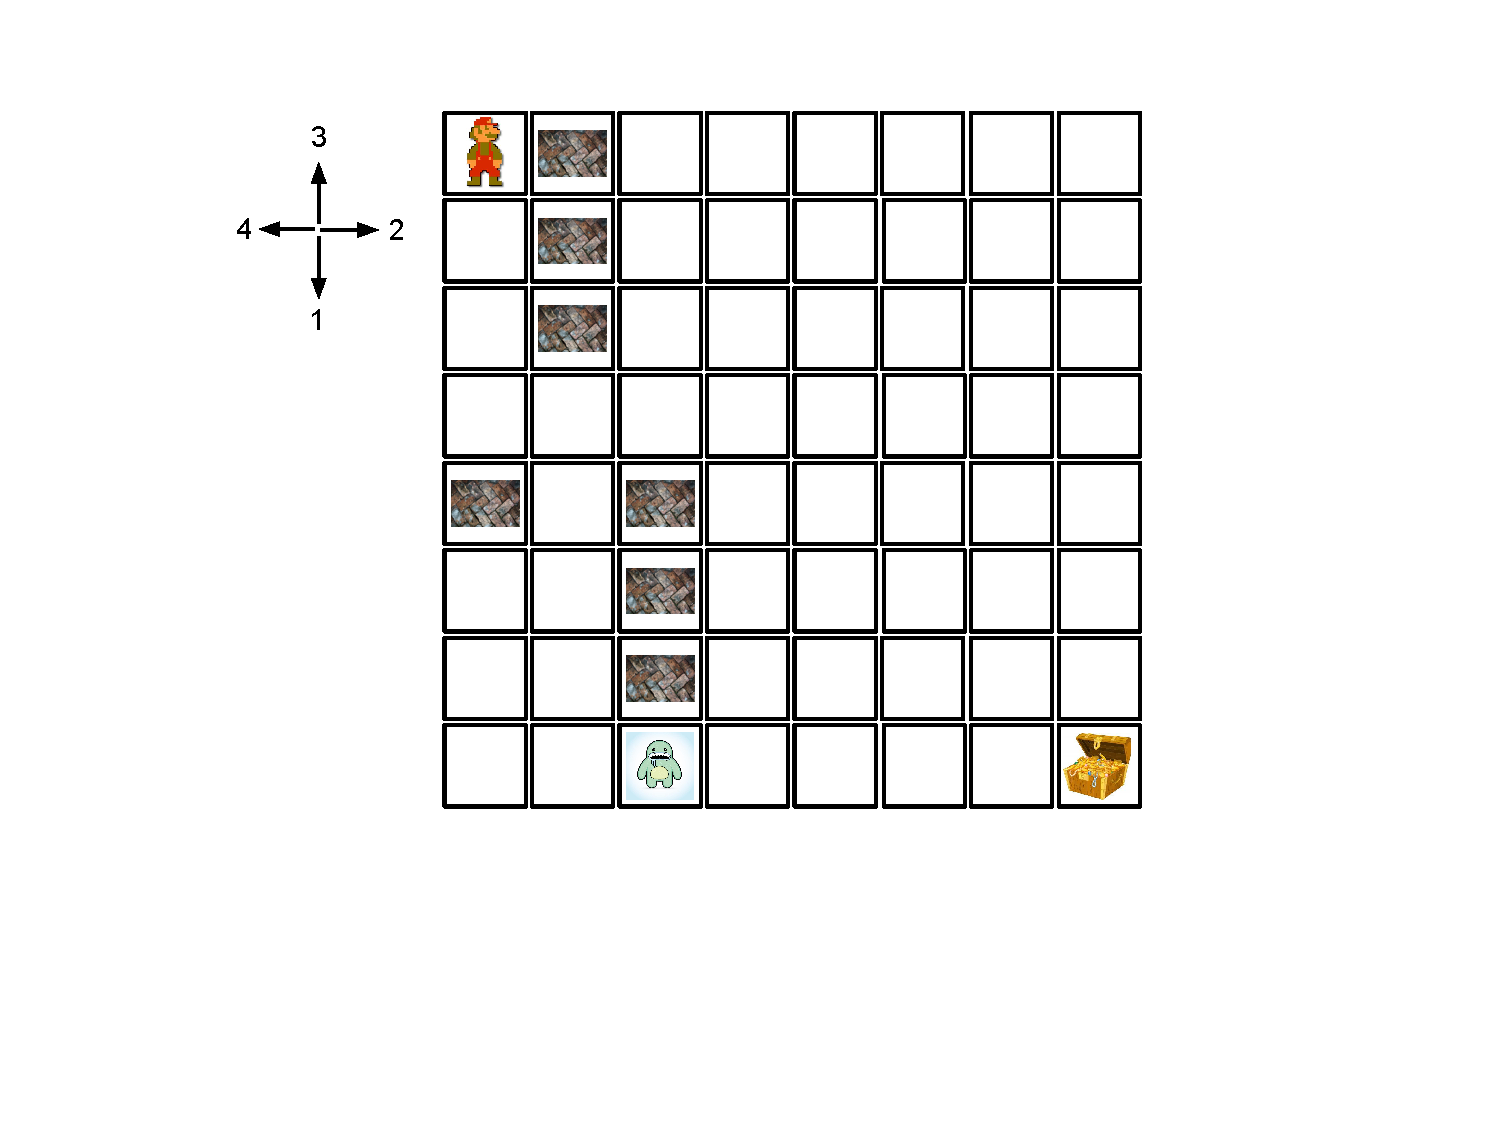
\includegraphics[width=12cm]{images/lab_00}
\end{frame}

\begin{frame}[fragile]
\frametitle{Задачата}
%\vspace*{-25pt}
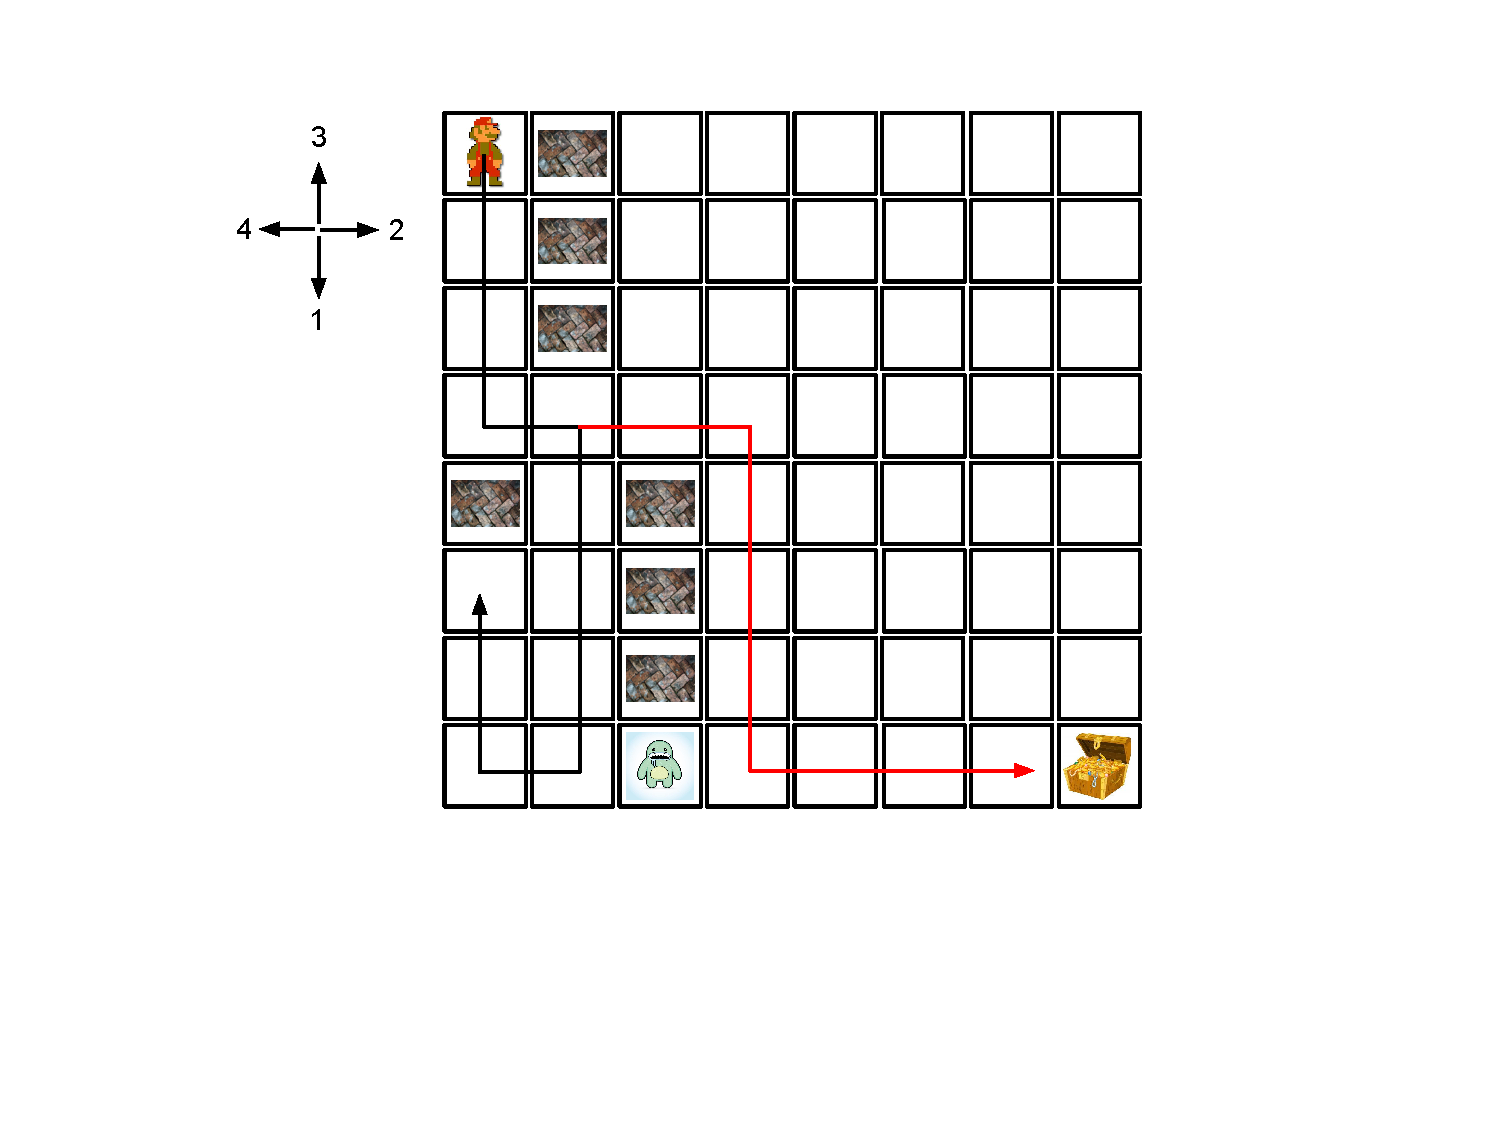
\includegraphics[width=12cm]{images/lab_sol}
\end{frame}


\begin{frame}[fragile]
\frametitle{Подзадача}
%\vspace*{-25pt}
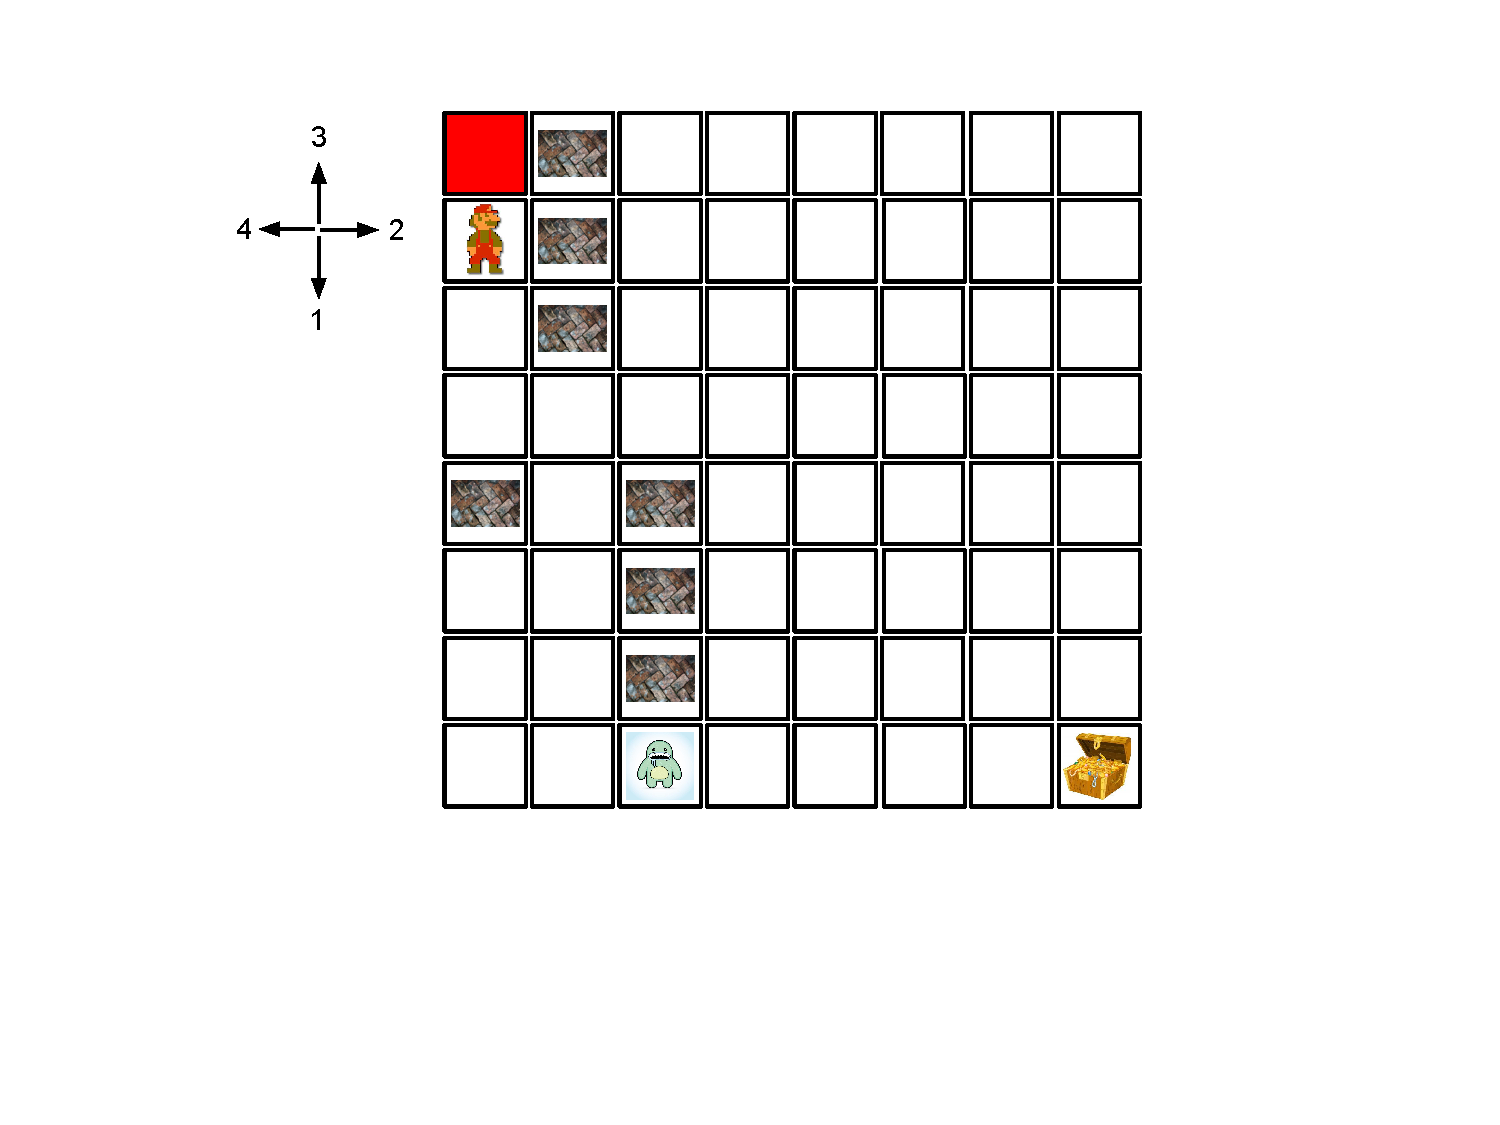
\includegraphics[width=12cm]{images/lab_01}
\end{frame}

\begin{frame}[fragile]
\frametitle{Търсене}
%\vspace*{-25pt}
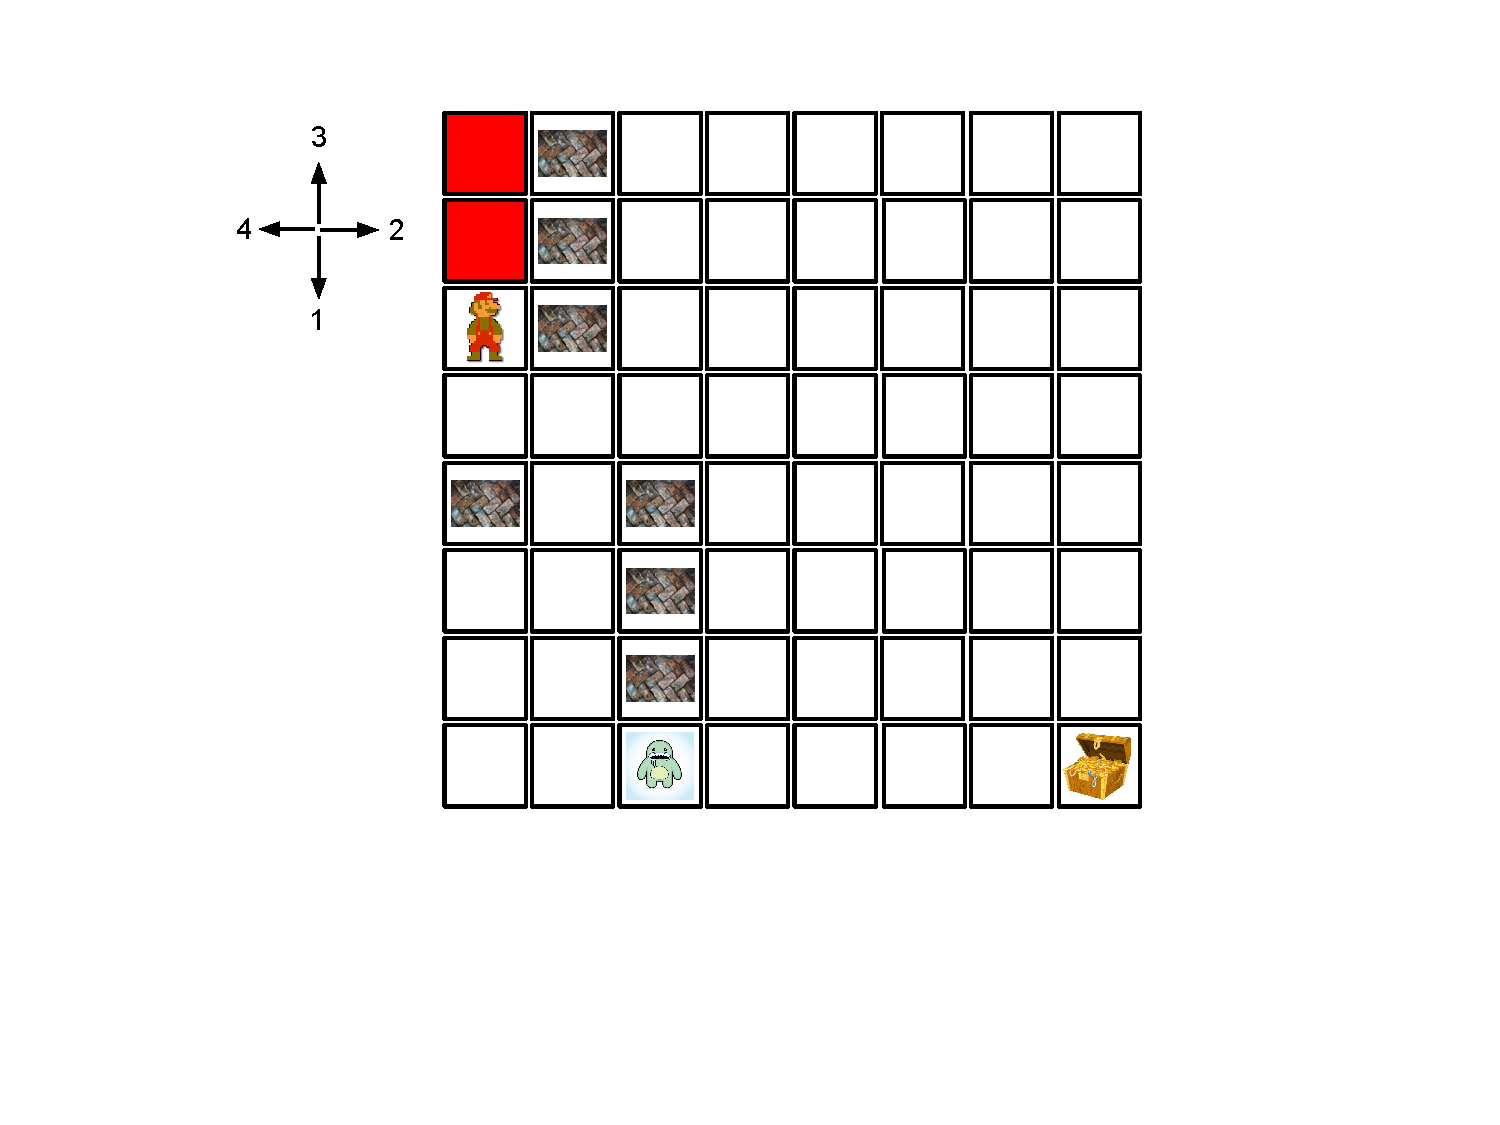
\includegraphics[width=12cm]{images/lab_02}
\end{frame}


\begin{frame}[fragile]
\frametitle{Търсене}
%\vspace*{-25pt}
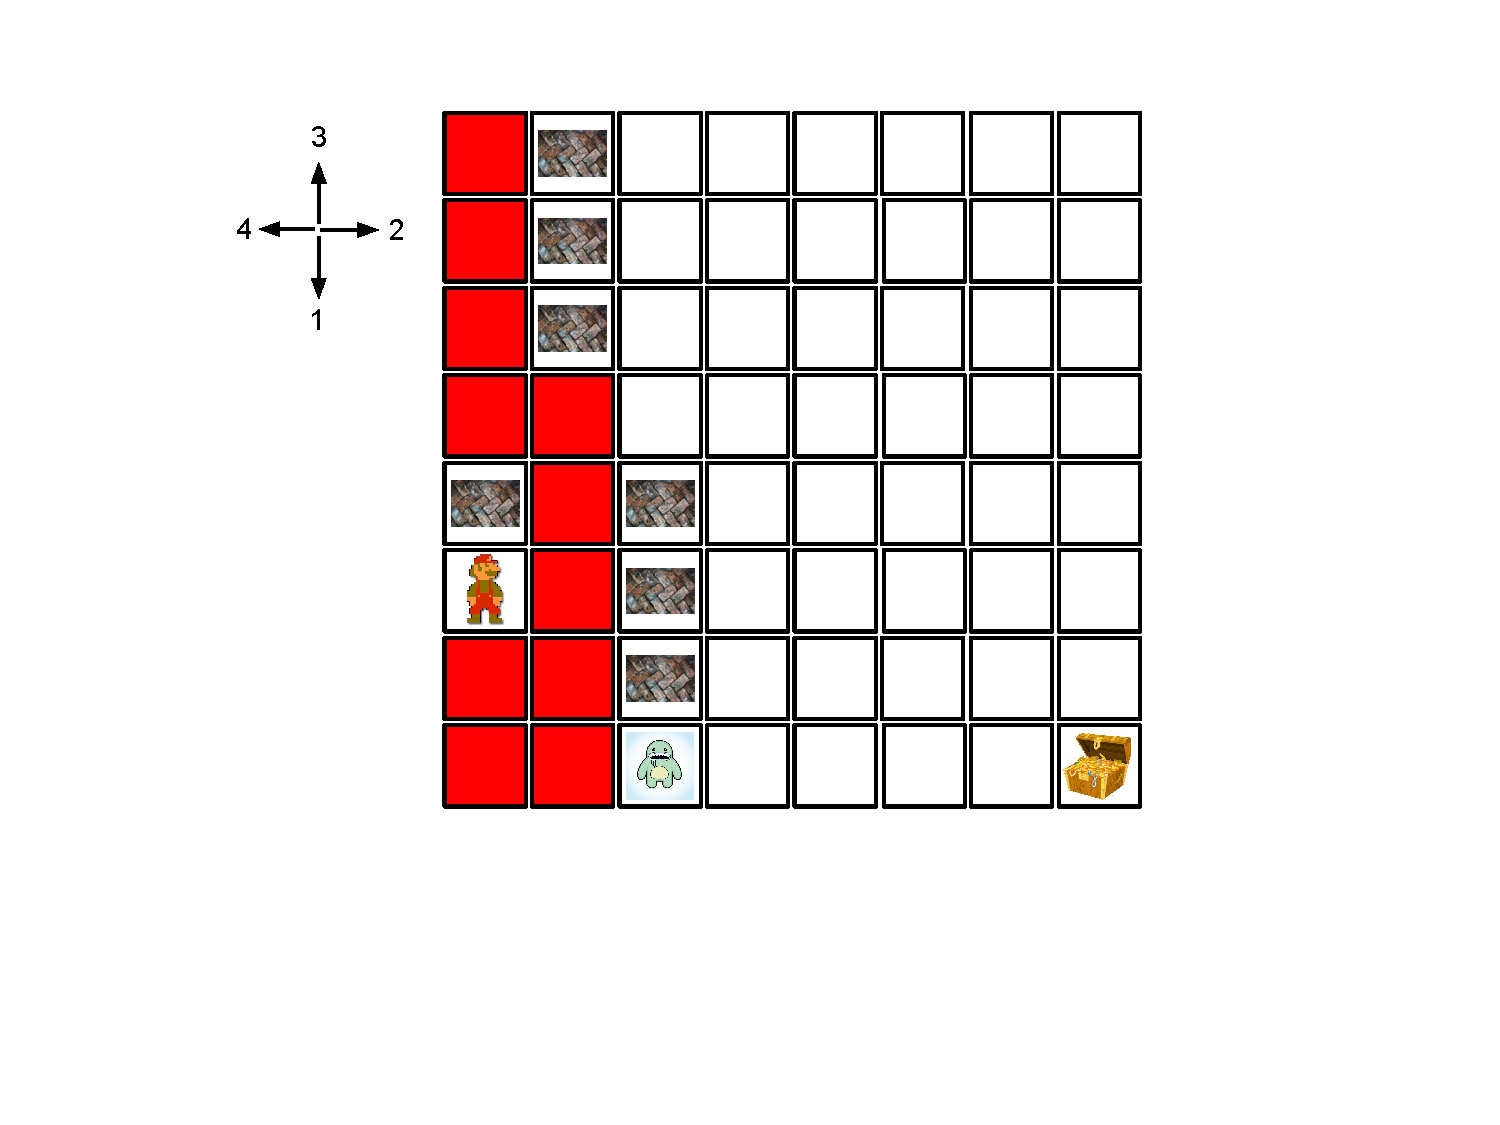
\includegraphics[width=12cm]{images/lab_dead1}
\end{frame}



\begin{frame}[fragile]
\frametitle{Търсене}
%\vspace*{-25pt}
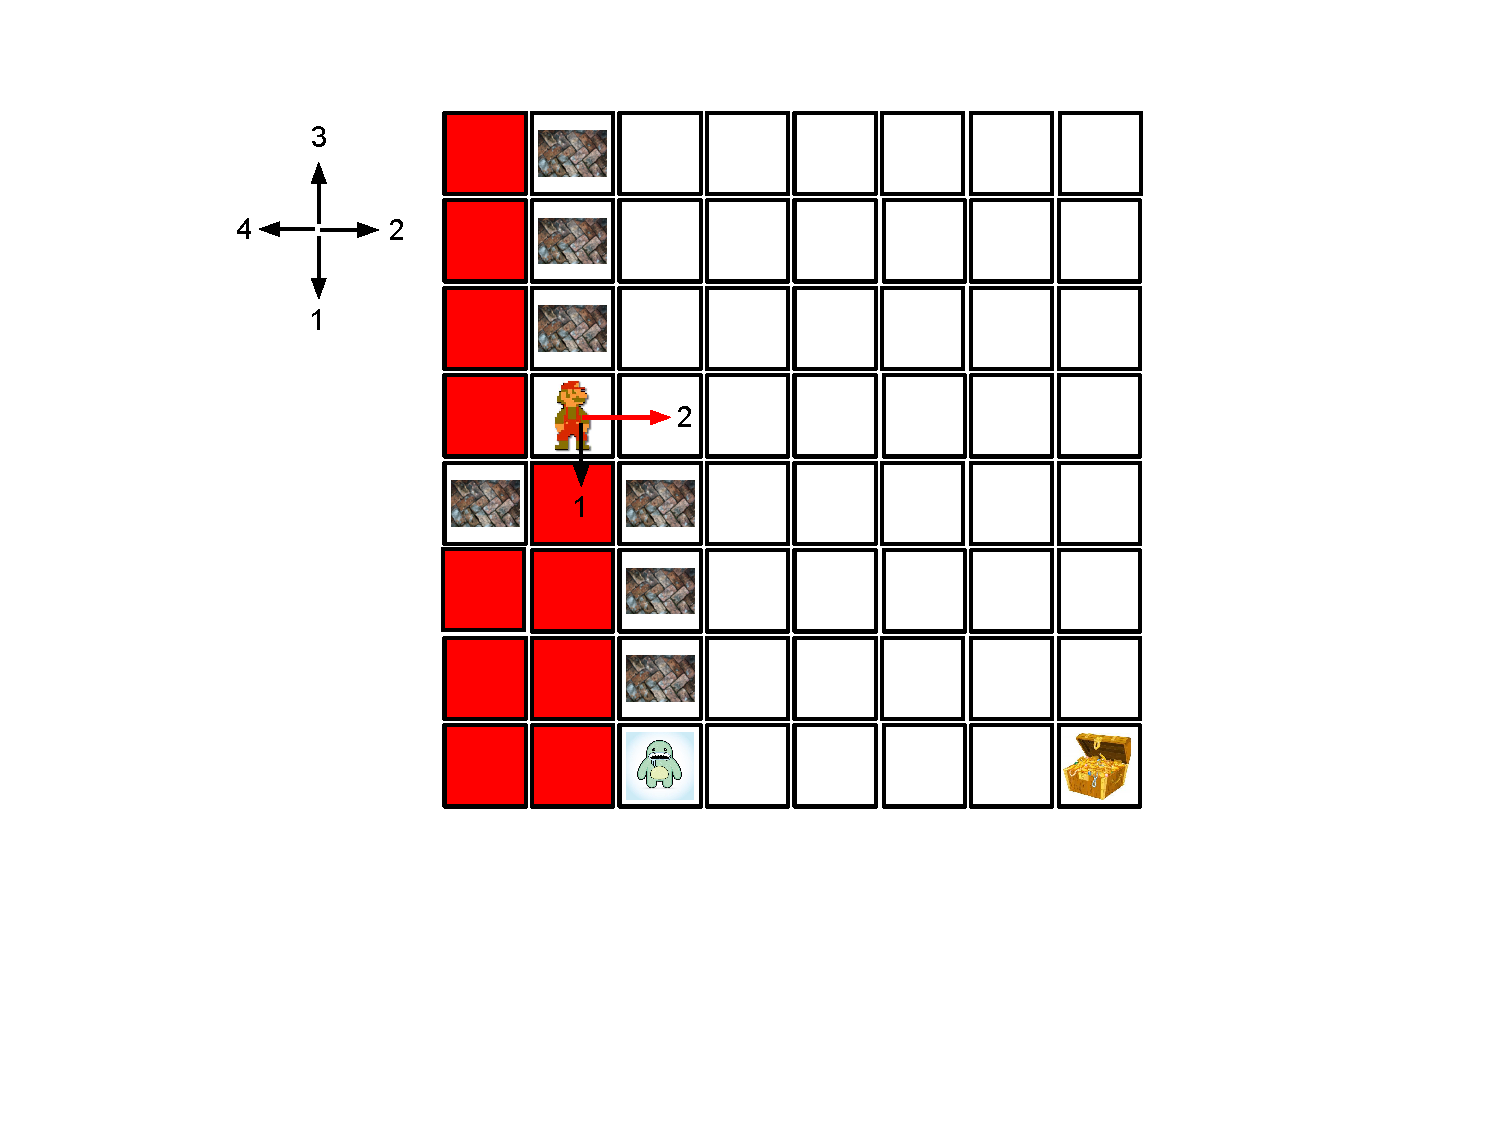
\includegraphics[width=12cm]{images/lab_choice_01}
\end{frame}


\begin{frame}[fragile]
\frametitle{Търсене}
%\vspace*{-25pt}
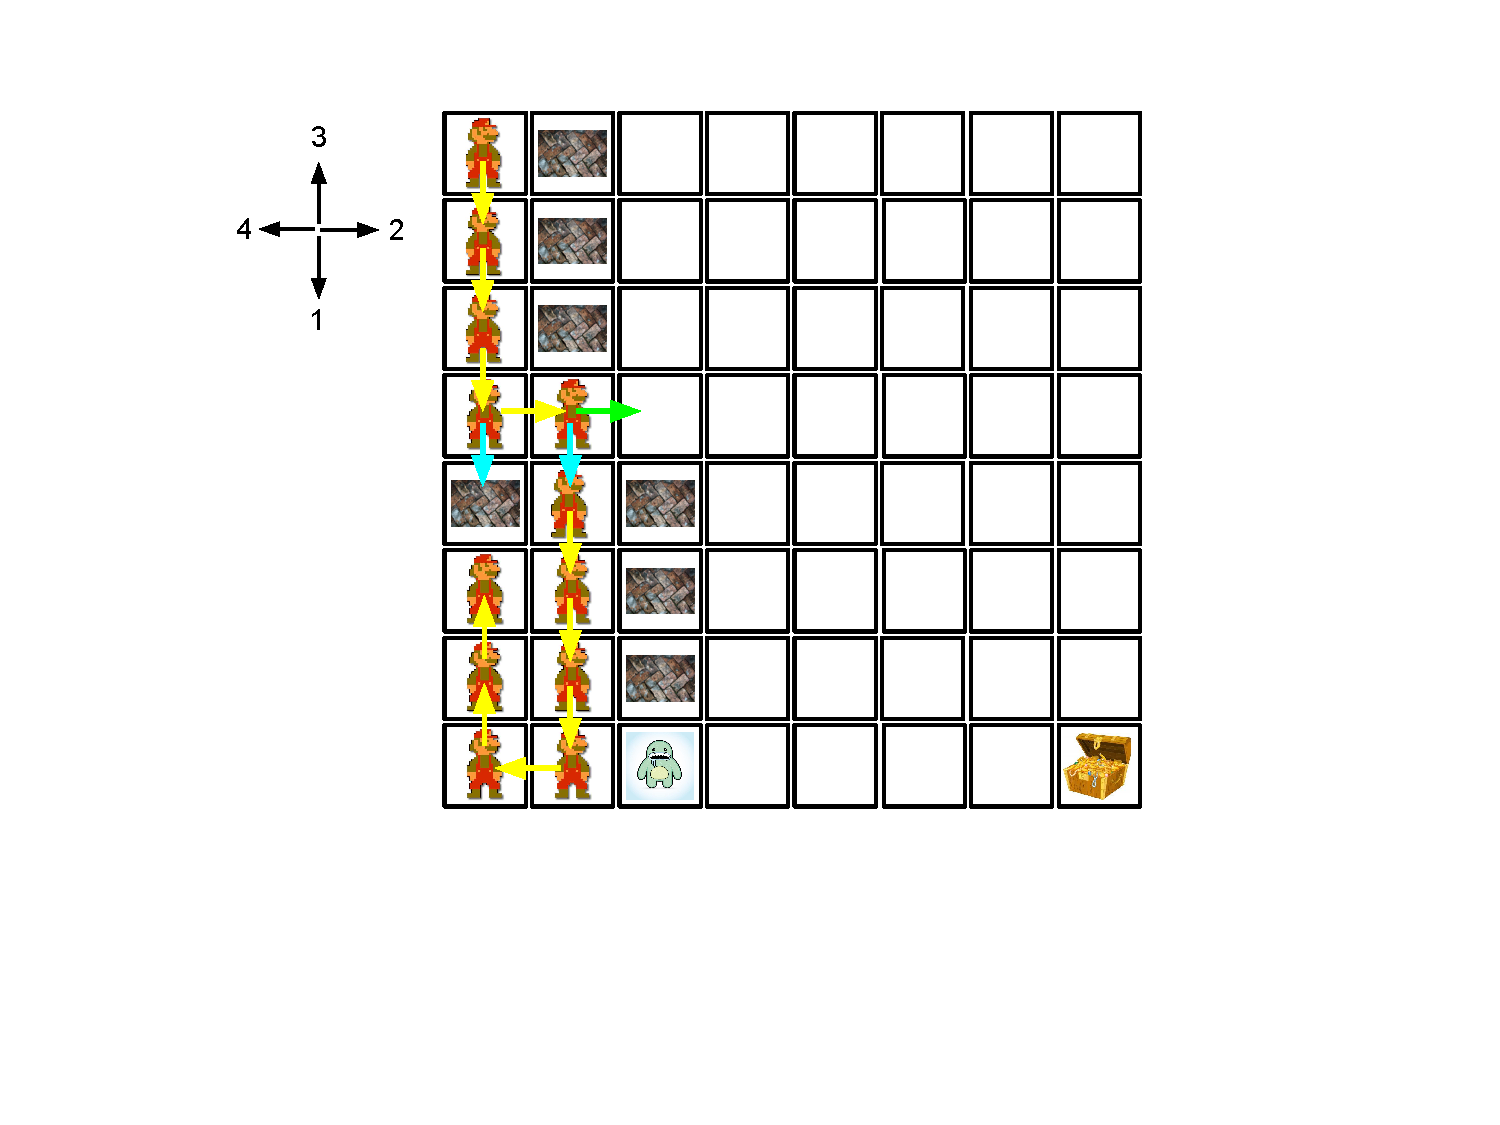
\includegraphics[width=12cm]{images/lab_st_02}
\end{frame}


\begin{frame}[fragile]
\frametitle{Търсене}
%\vspace*{-25pt}
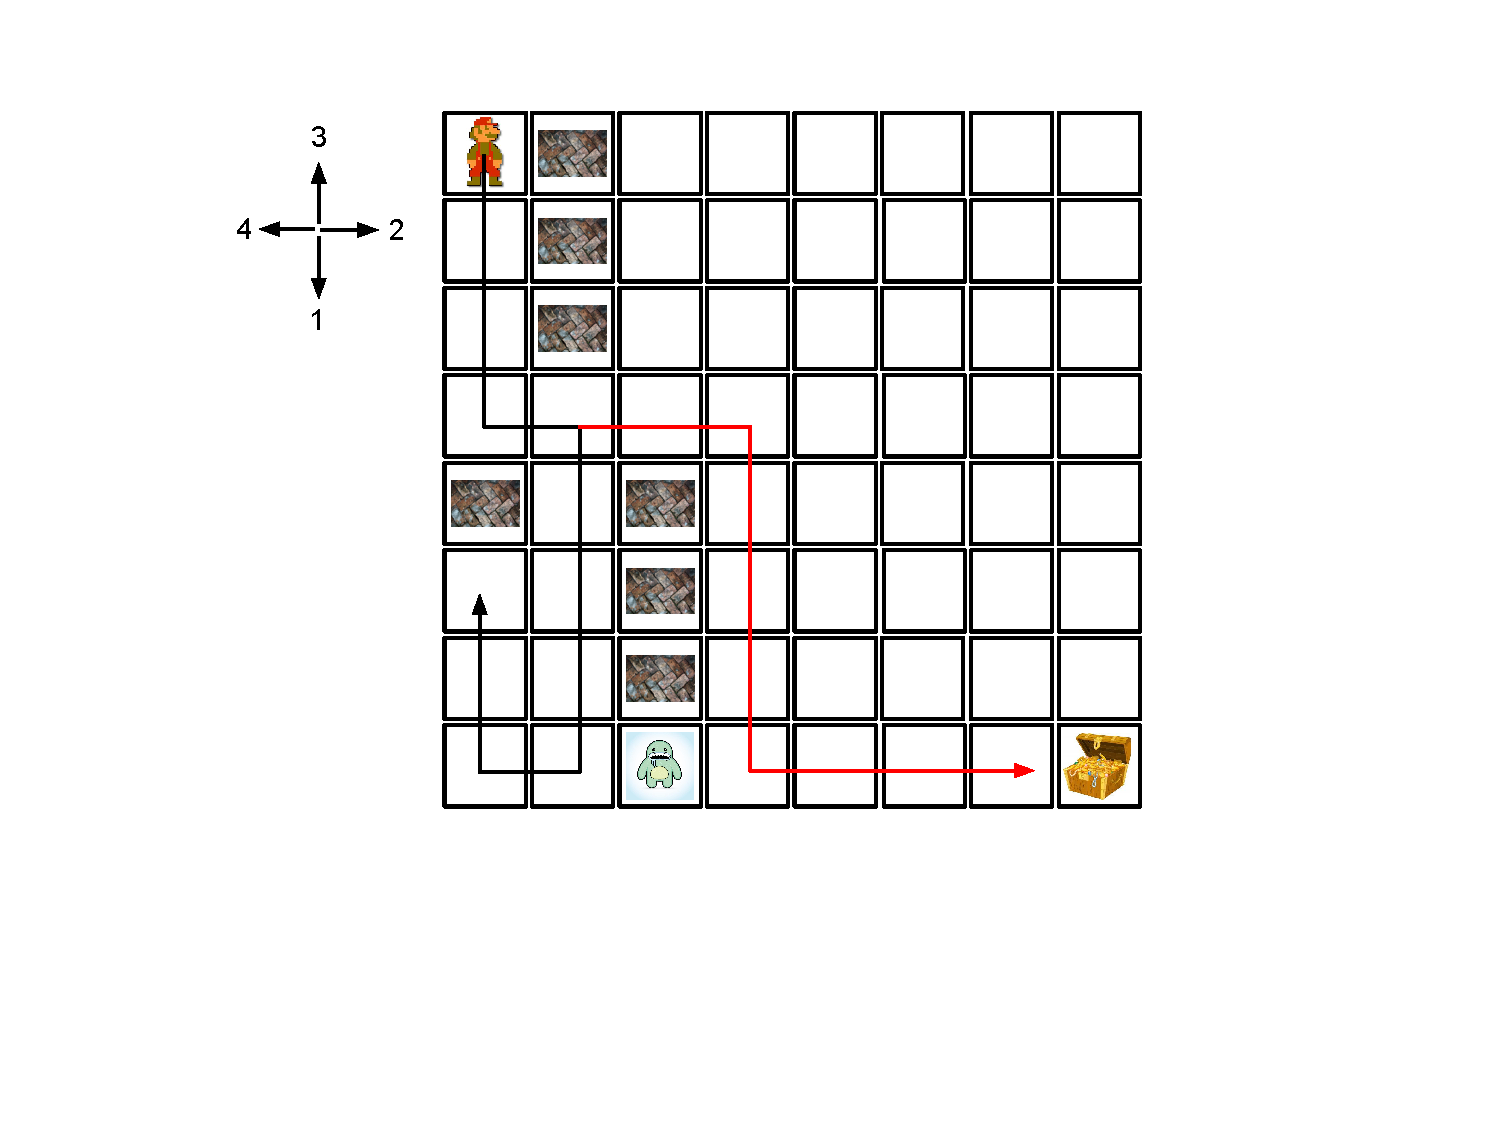
\includegraphics[width=12cm]{images/lab_sol}
\end{frame}


\begin{frame}[fragile]
\frametitle{Модел на лабиринта}
\relscale{1.0}
\begin{lstlisting}
  const int ls = 8; 
  int lab[ls][ls] = {0,1,0,0,0,0,0,0,
                     0,1,0,0,0,0,0,0,
                     0,1,0,0,0,0,0,0,
                     0,0,0,0,0,0,0,0,
                     1,0,1,0,0,0,0,0,
                     0,0,1,0,0,0,0,0,
                     0,0,1,0,0,0,0,0,
                     0,0,2,0,0,0,0,0};
\end{lstlisting}

\end{frame}


\begin{frame}[fragile]
\frametitle{Модел на лабиринта}
\relscale{0.8}
\begin{lstlisting}
void markVisited (int lab[ls][ls], int row, int col)
{
  lab[row][col] = 9;
}

bool canStepOn (int lab[ls][ls], int row, int col)
{
  return row >= 0 &&
         col >= 0 && 
         row < ls &&
         col < ls &&
         lab[row][col] == 0;
}
\end{lstlisting}

\end{frame}


\begin{frame}[fragile]
\frametitle{Проби и грешки}
\relscale{0.7}
\begin{lstlisting}
bool wayExists  (int lab[ls][ls], int startRow, int startCol)
{
  if (startRow == ls-1 && startCol == ls-1)
  { return true; }

  markVisited (lab,startRow,startCol);

  if (canStepOn (lab,startRow+1,startCol) && 
      wayExists (lab,startRow+1,startCol))
        return true;
  if (canStepOn (lab,startRow,startCol+1) && 
      wayExists (lab,startRow,startCol+1))
        return true;
  if (canStepOn (lab,startRow-1,startCol) && 
      wayExists (lab,startRow-1,startCol))
        return true;
  if (canStepOn (lab,startRow,startCol-1) && 
      wayExists (lab,startRow,startCol-1))
        return true;
  return false;
}
\end{lstlisting}
\end{frame}



\begin{frame}[fragile]
\frametitle{Проби и грешки}
\vspace{-20px}
\begin{flushright}
  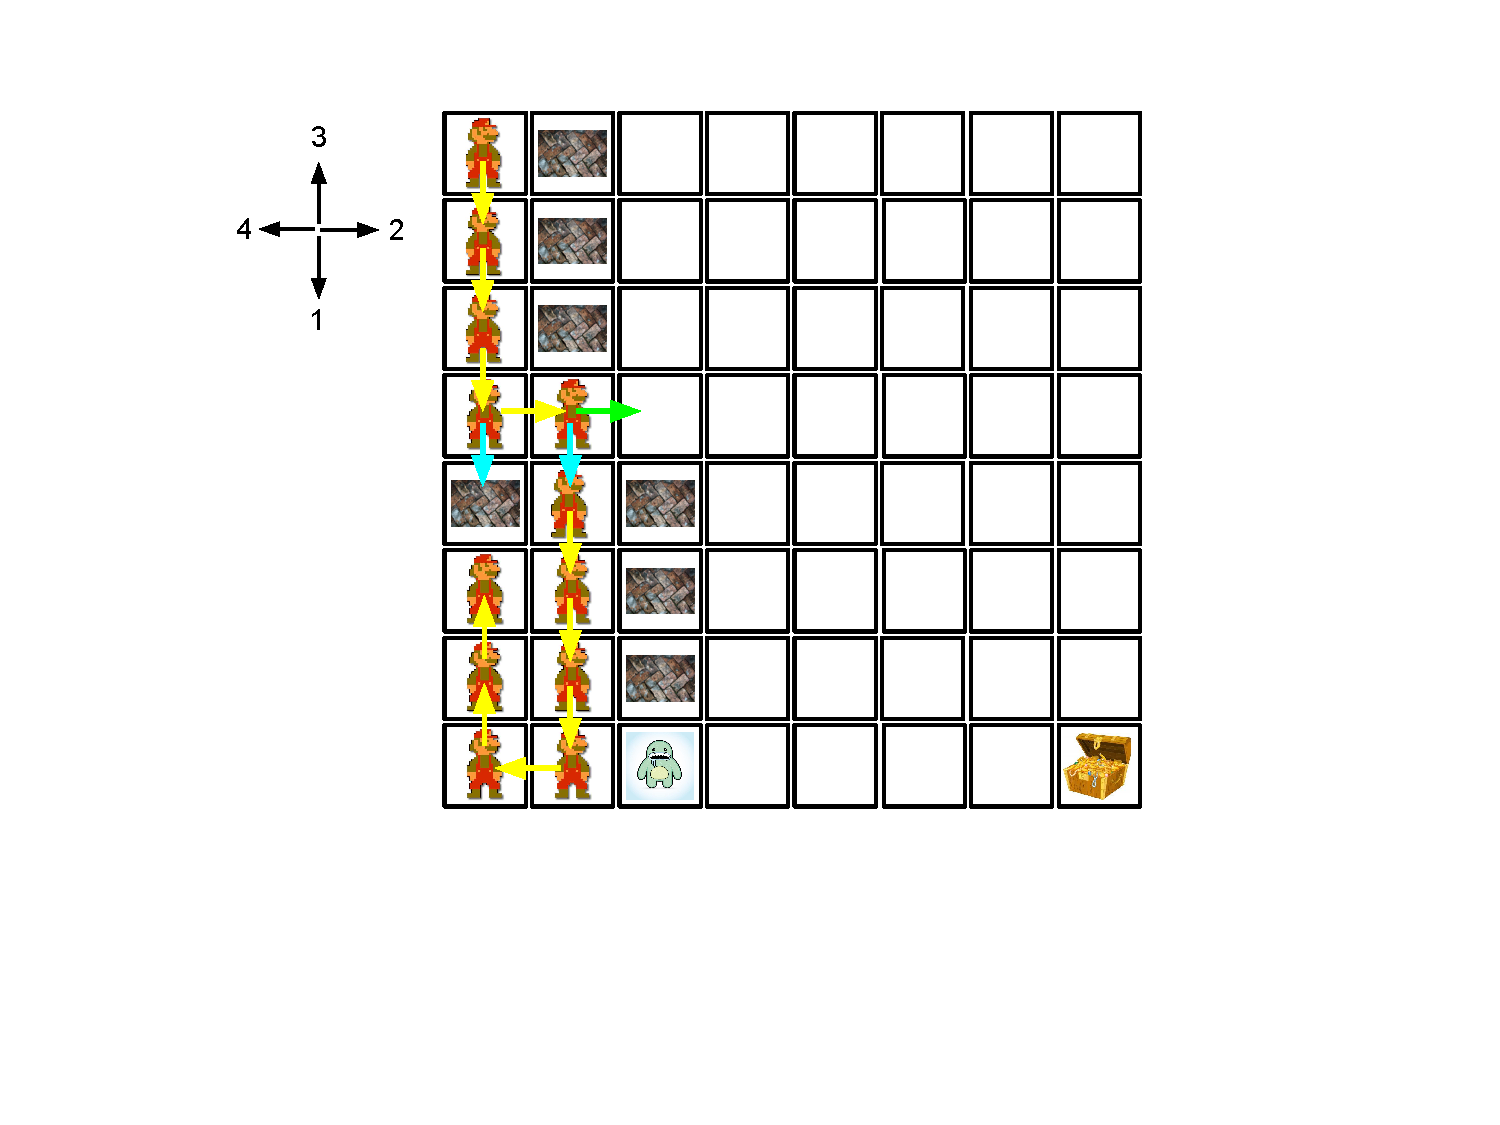
\includegraphics[width=10cm]{images/lab_st_02}
\end{flushright}
\vspace{-60px}
\relscale{0.7}
\begin{lstlisting}
  if (canStepOn (lab,startRow+1,startCol) && 
      wayExists (lab,startRow+1,startCol))
        return true;
  if (canStepOn (lab,startRow,startCol+1) && 
      wayExists (lab,startRow,startCol+1))
        return true;
...
\end{lstlisting}
\end{frame}


\section{Царици}

\begin{frame}
\centerline{Пъзел с 8 царици}
\end{frame}

\begin{frame}[fragile]
\frametitle{Задачата}
%\vspace*{-25pt}
\begin{center}
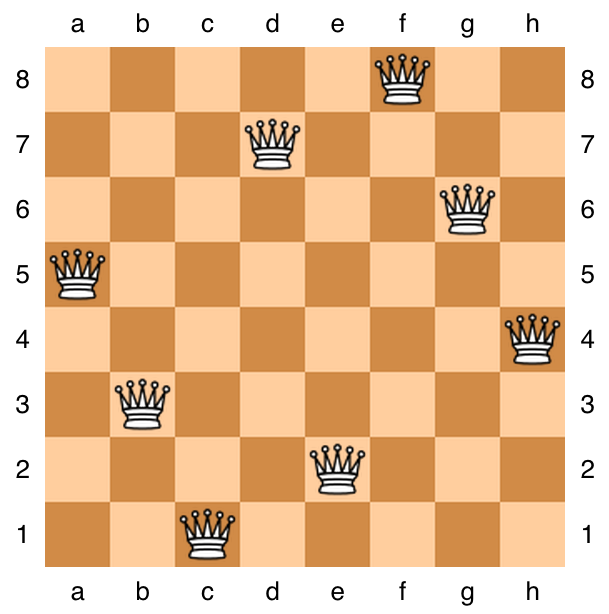
\includegraphics[width=7cm]{images/puzzle}
\end{center}
\end{frame}



\begin{frame}[fragile]
\frametitle{Търсене}
%\vspace*{-25pt}
\begin{center}
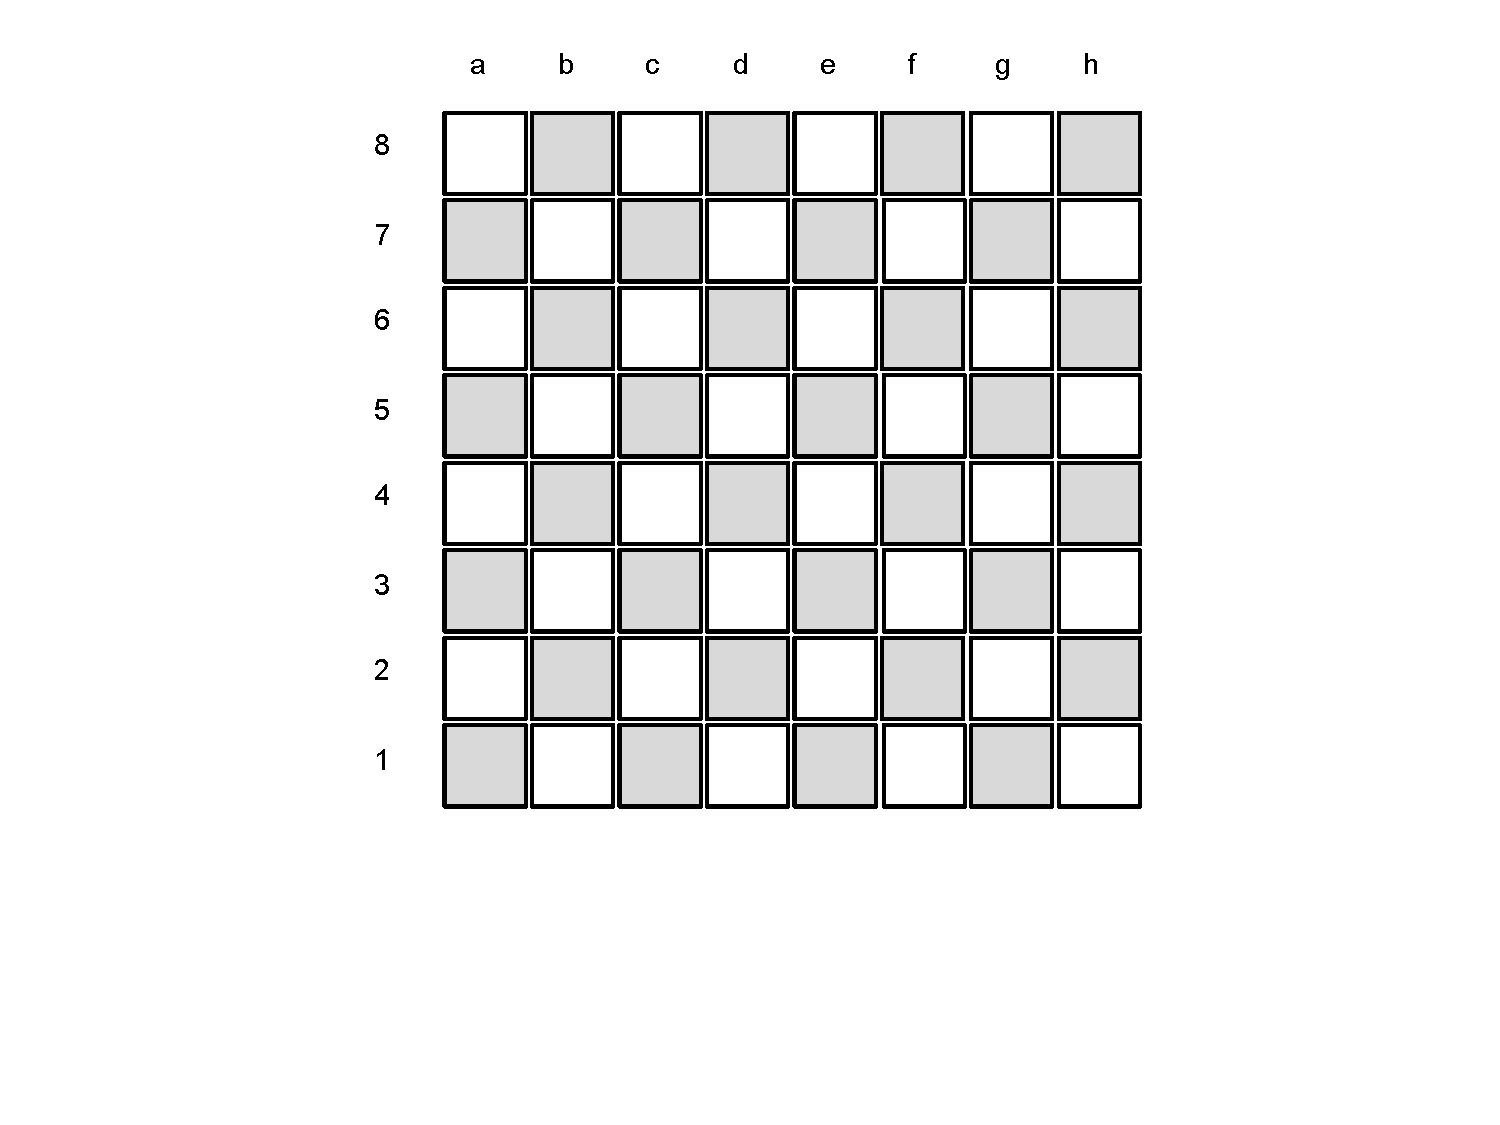
\includegraphics[width=12cm]{images/cb_00}
\end{center}
\end{frame}

\begin{frame}[fragile]
\frametitle{Търсене}
%\vspace*{-25pt}
\begin{center}
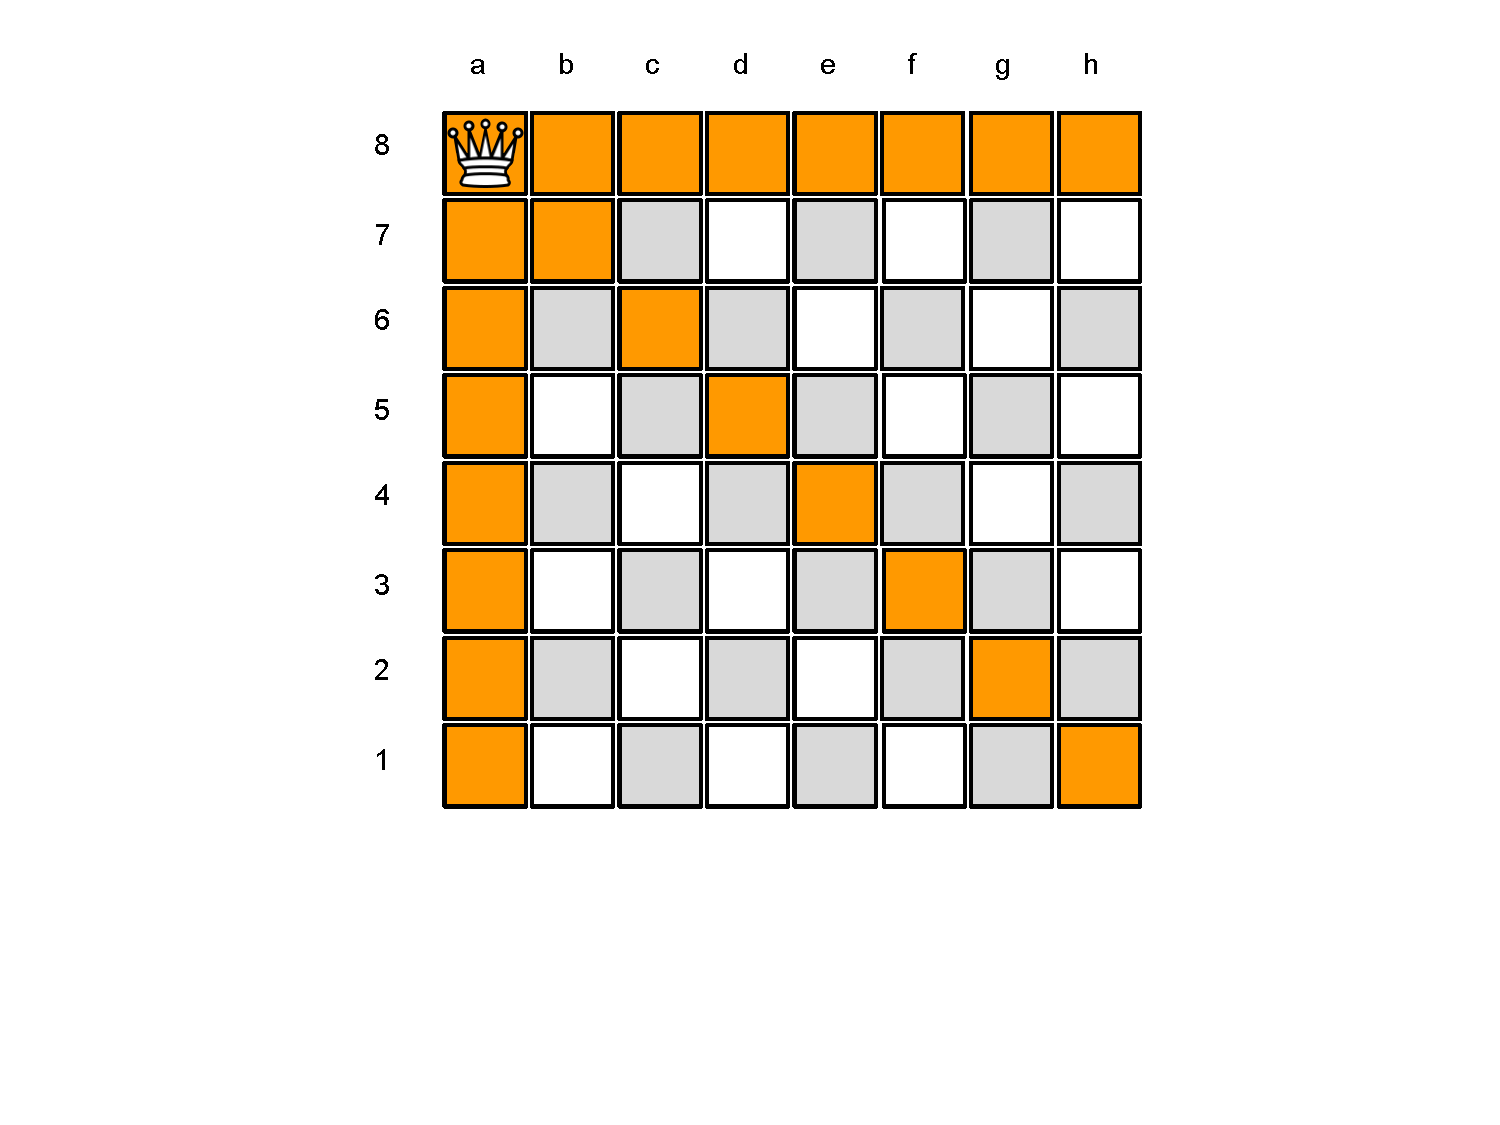
\includegraphics[width=12cm]{images/cb_01}
\end{center}
\end{frame}

\begin{frame}[fragile]
\frametitle{Търсене}
%\vspace*{-25pt}
\begin{center}
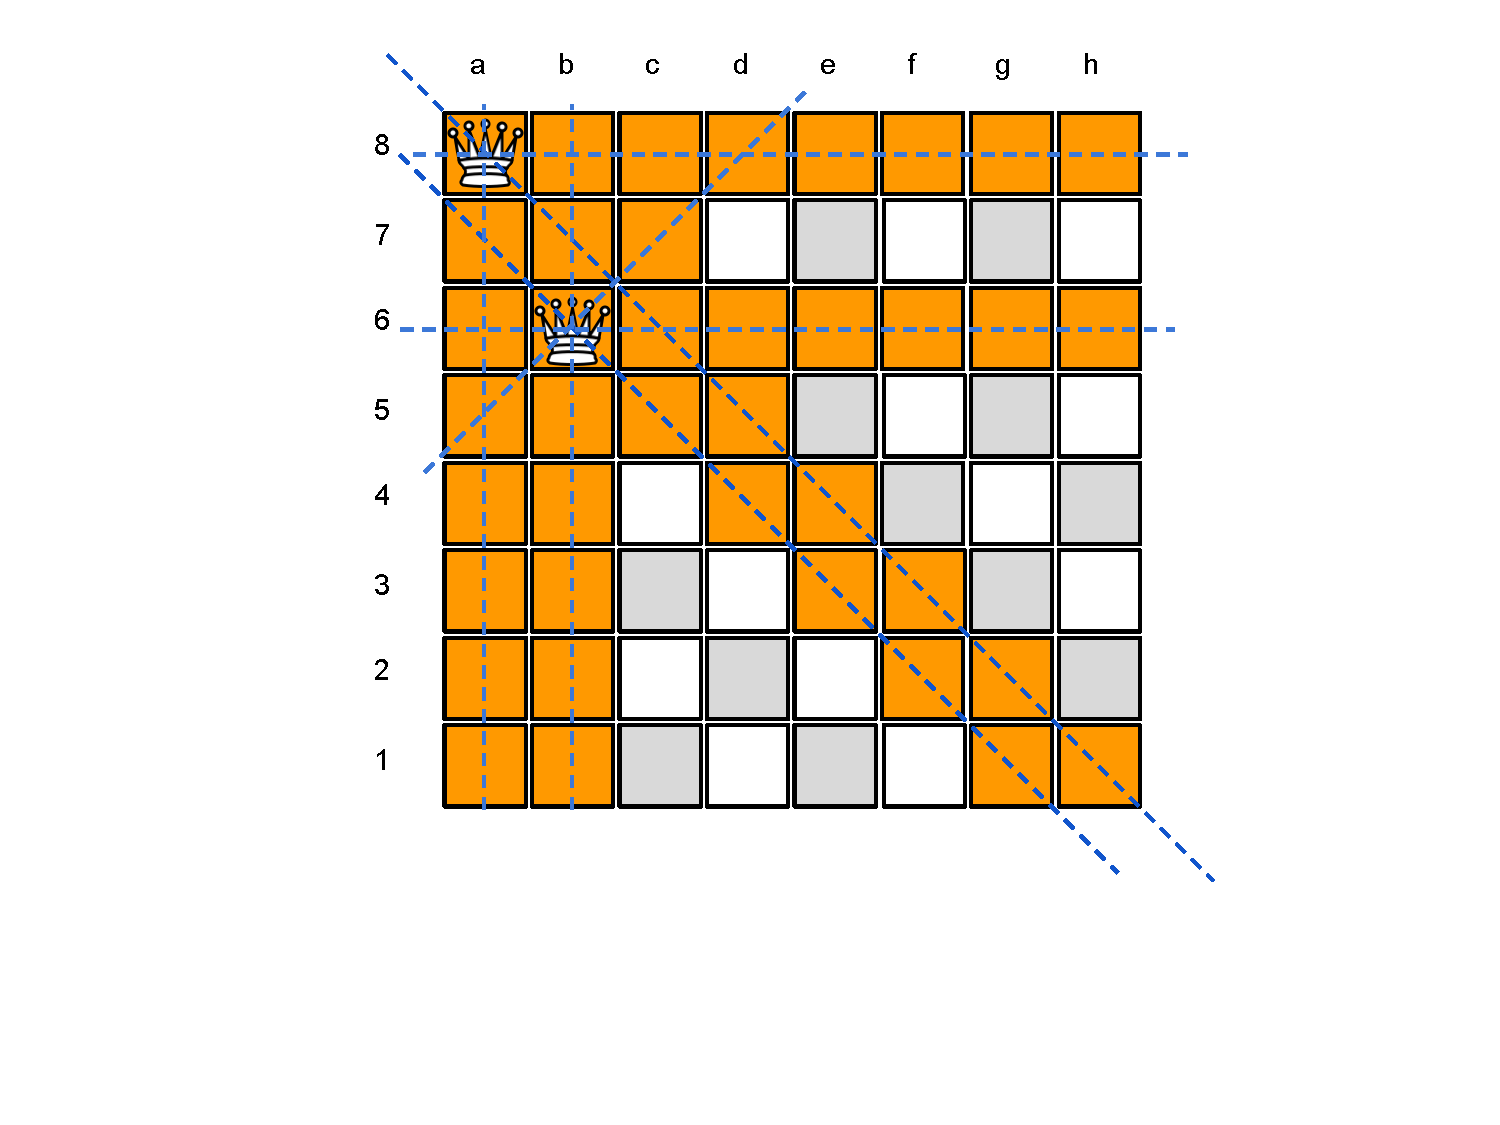
\includegraphics[width=12cm]{images/cb_02}
\end{center}
\end{frame}


\begin{frame}[fragile]
\frametitle{Търсене}
%\vspace*{-25pt}
\begin{center}
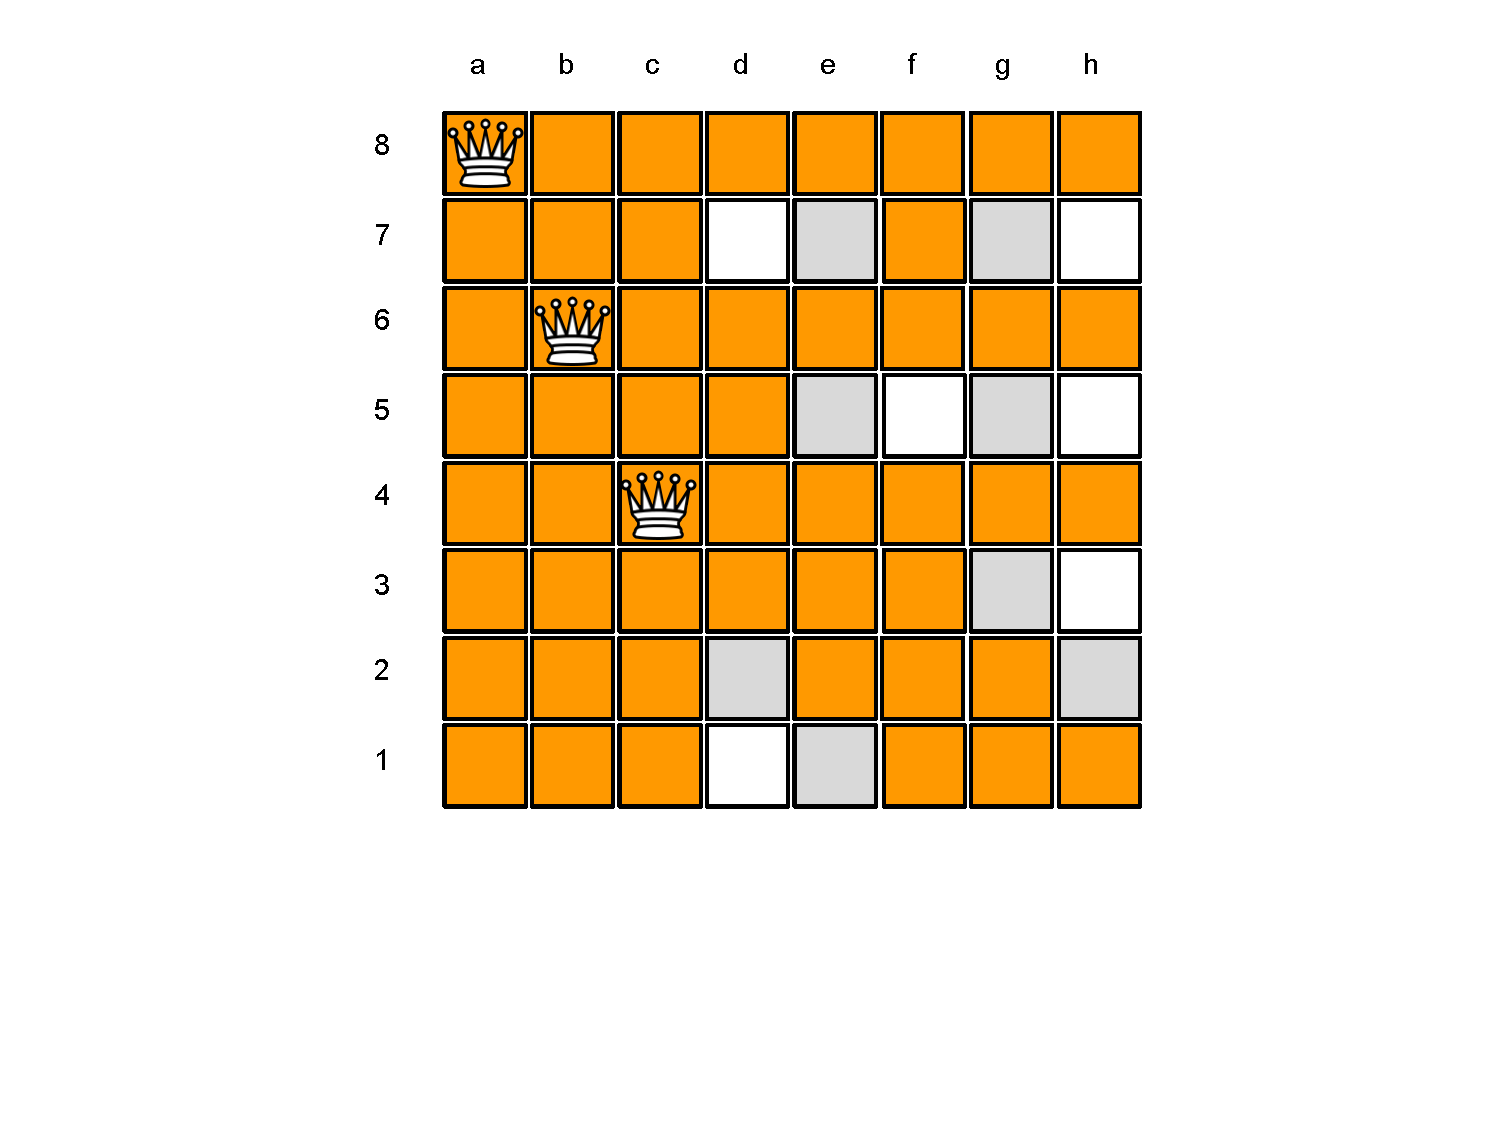
\includegraphics[width=12cm]{images/cb_03}
\end{center}
\end{frame}


\begin{frame}[fragile]
\frametitle{Търсене}
%\vspace*{-25pt}
\begin{center}
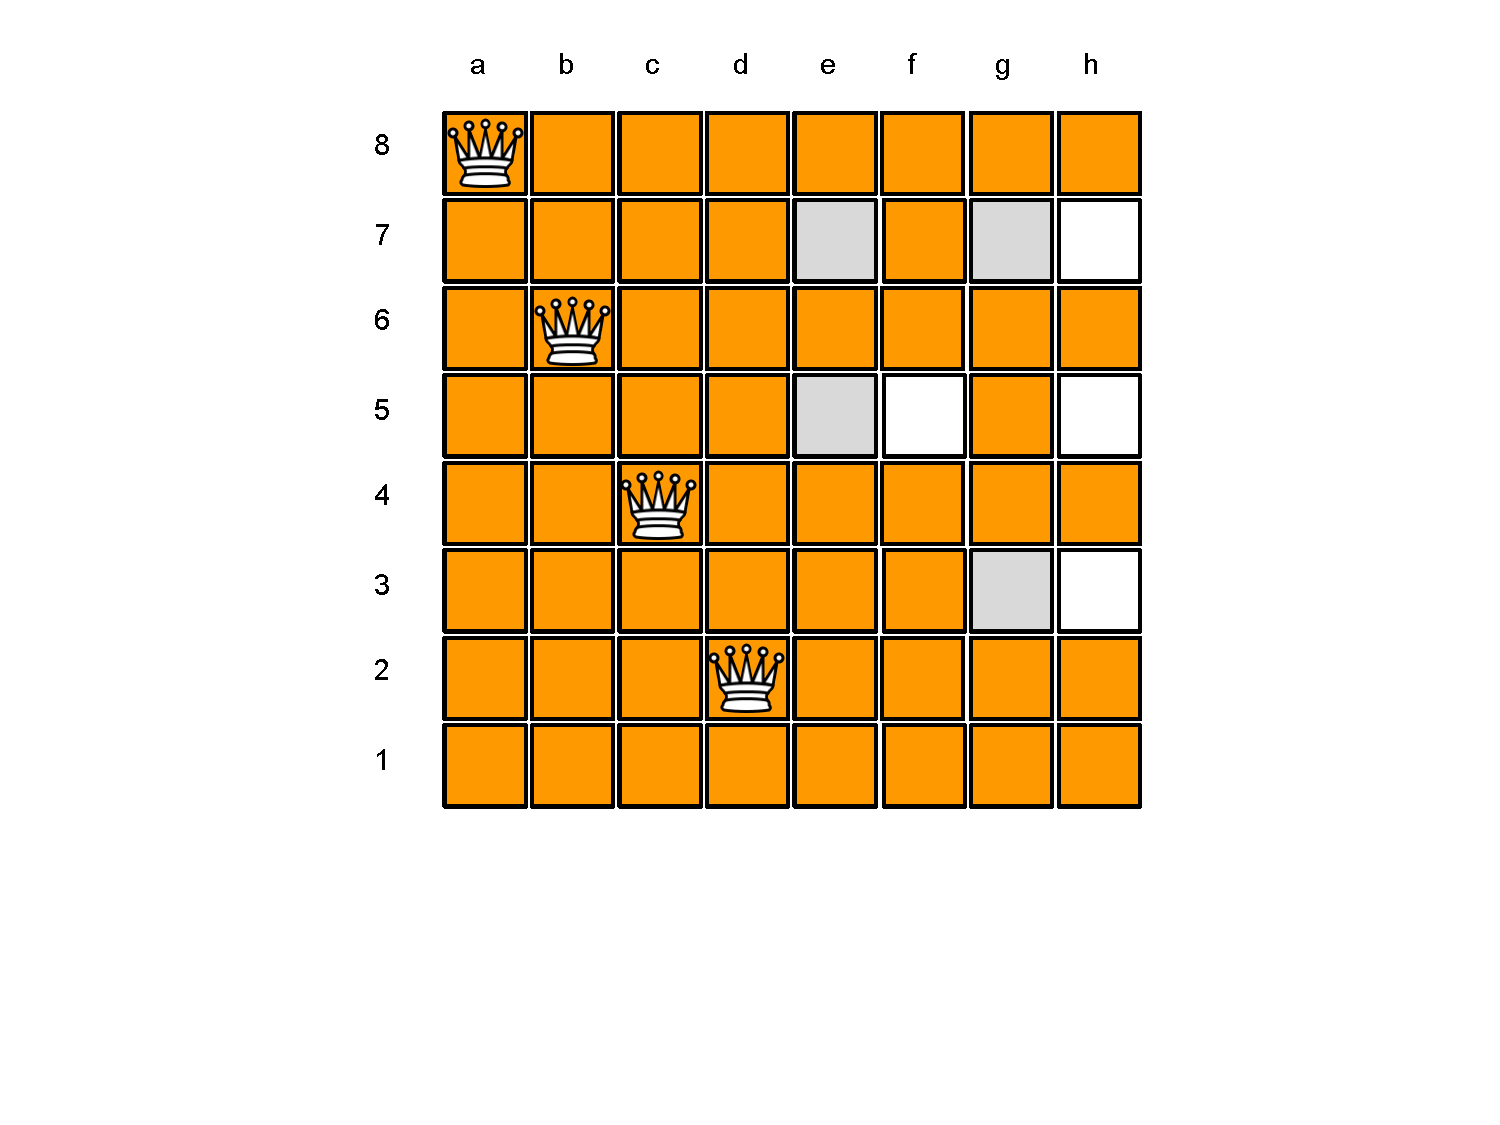
\includegraphics[width=12cm]{images/cb_04}
\end{center}
\end{frame}


\begin{frame}[fragile]
\frametitle{Търсене}
%\vspace*{-25pt}
\begin{center}
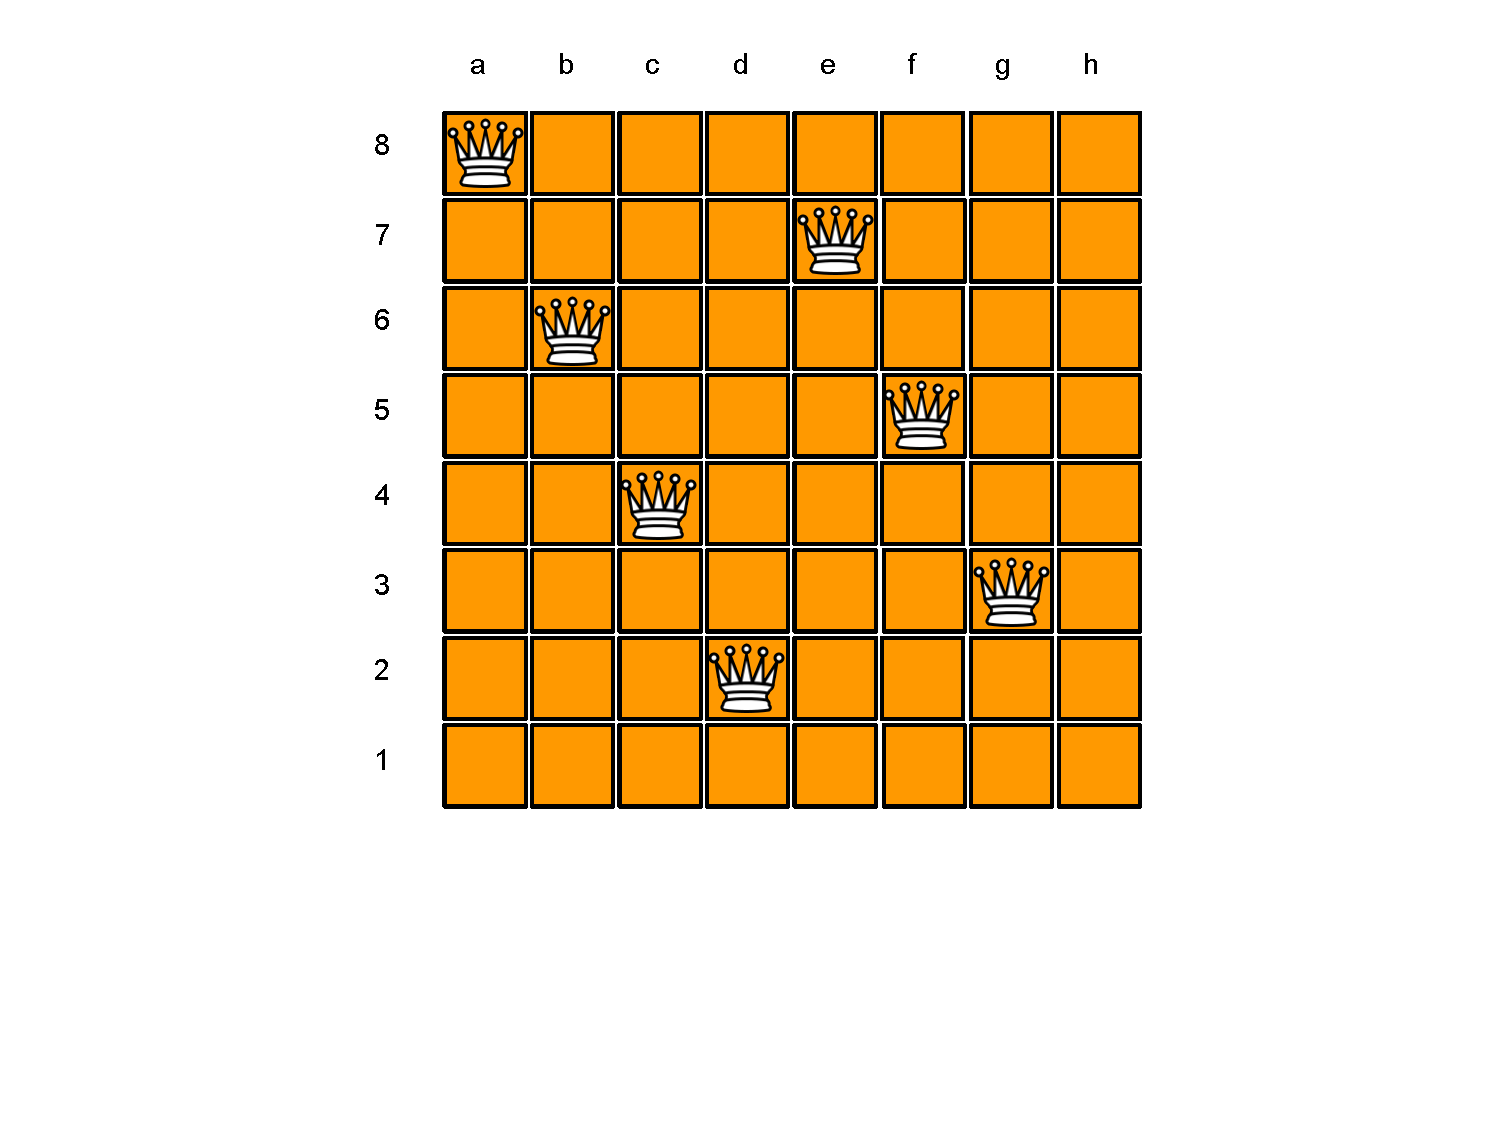
\includegraphics[width=12cm]{images/cb_07}
\end{center}
\end{frame}


\begin{frame}[fragile]
\frametitle{Подзадача}
%\vspace*{-25pt}
\begin{center}
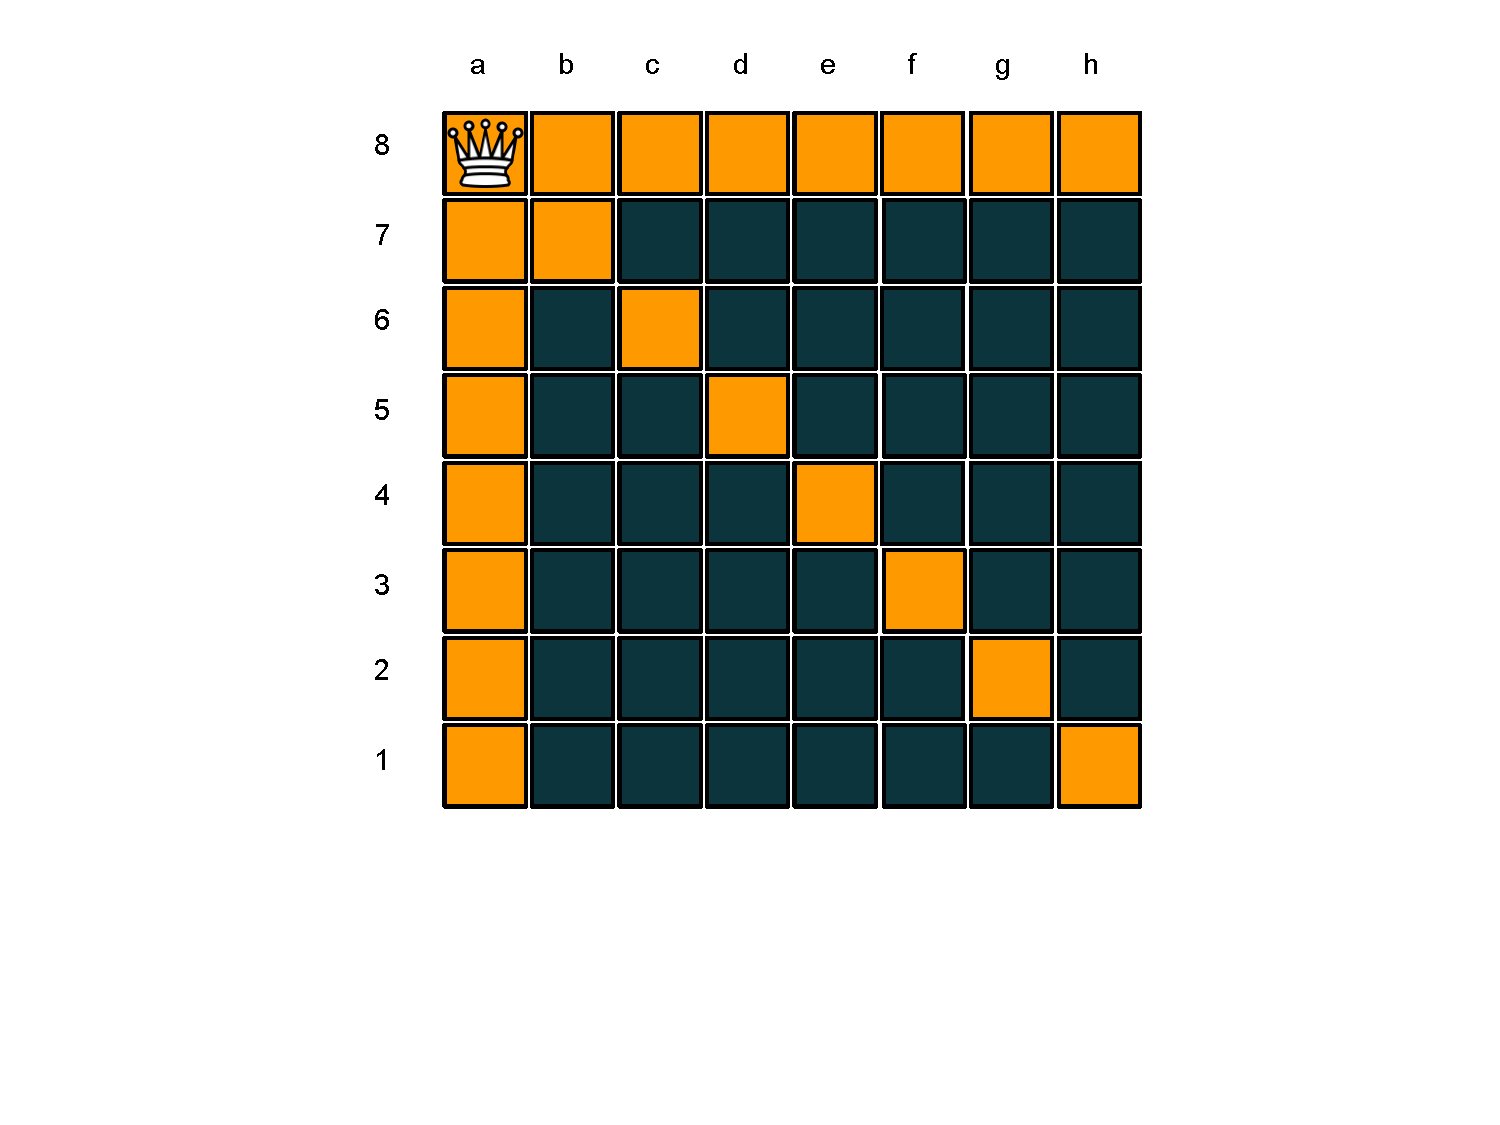
\includegraphics[width=12cm]{images/cb_0101}
\end{center}
\end{frame}


\begin{frame}[fragile]
\frametitle{Търсене}
%\vspace*{-25pt}
\begin{center}
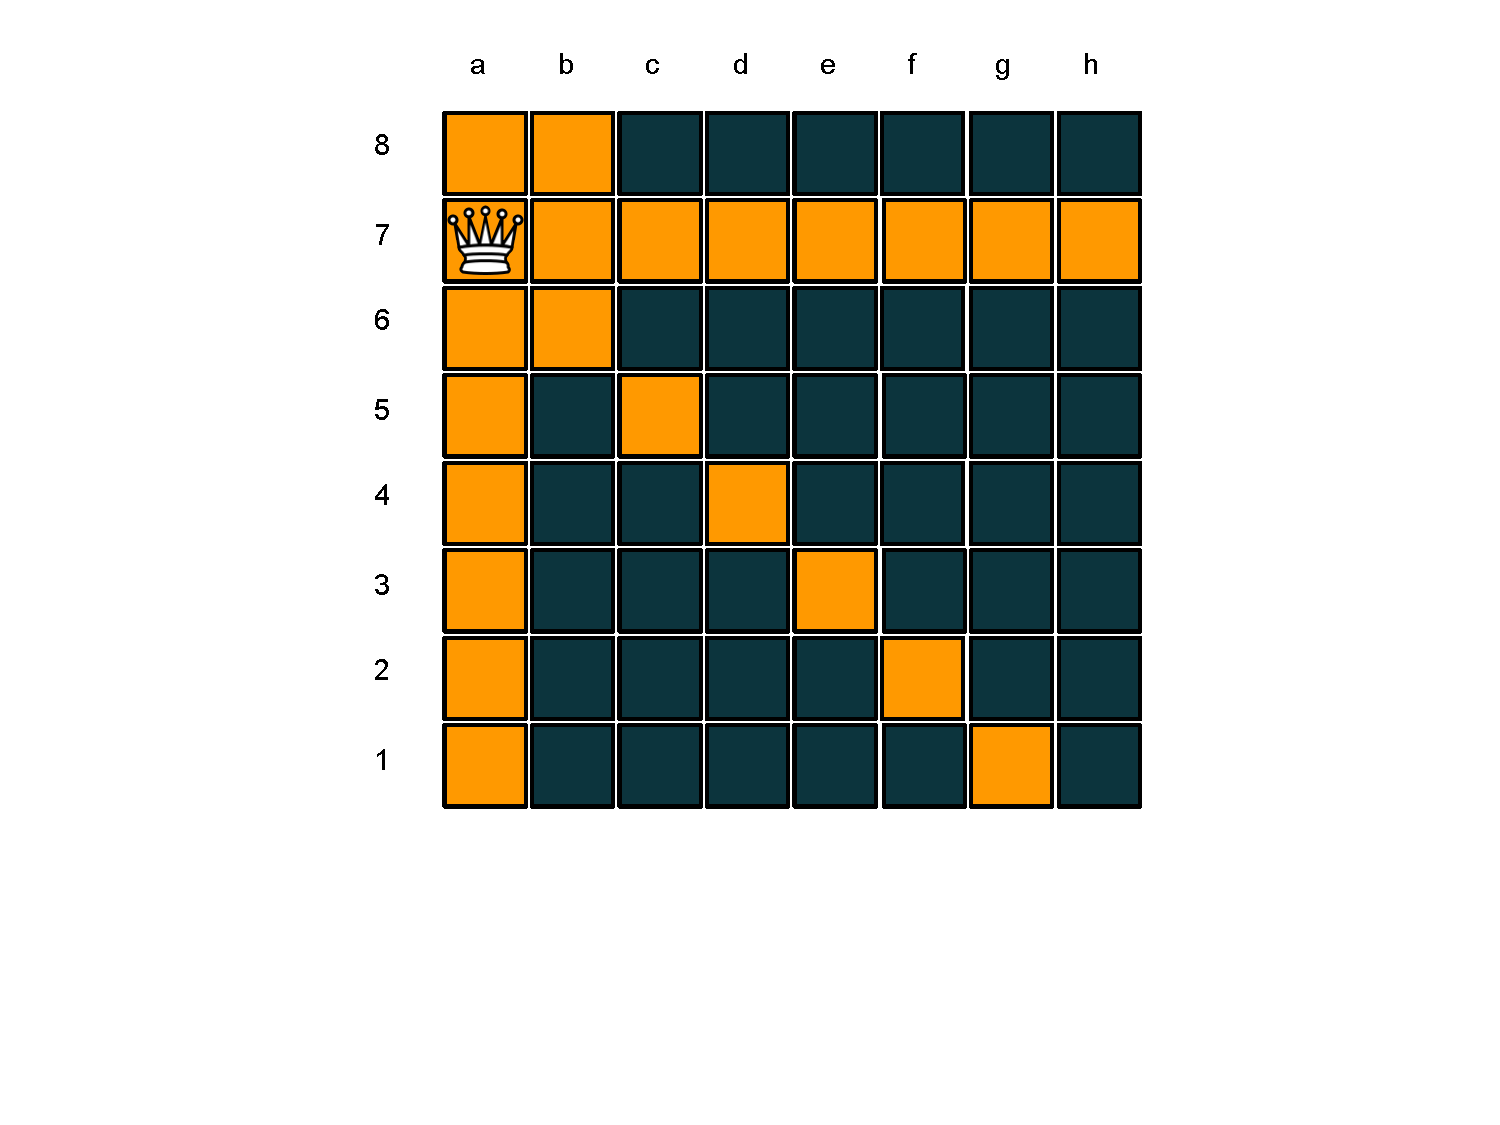
\includegraphics[width=12cm]{images/cb_0102}
\end{center}
\end{frame}


\begin{frame}[fragile]
\frametitle{Търсене}
%\vspace*{-25pt}
\begin{center}
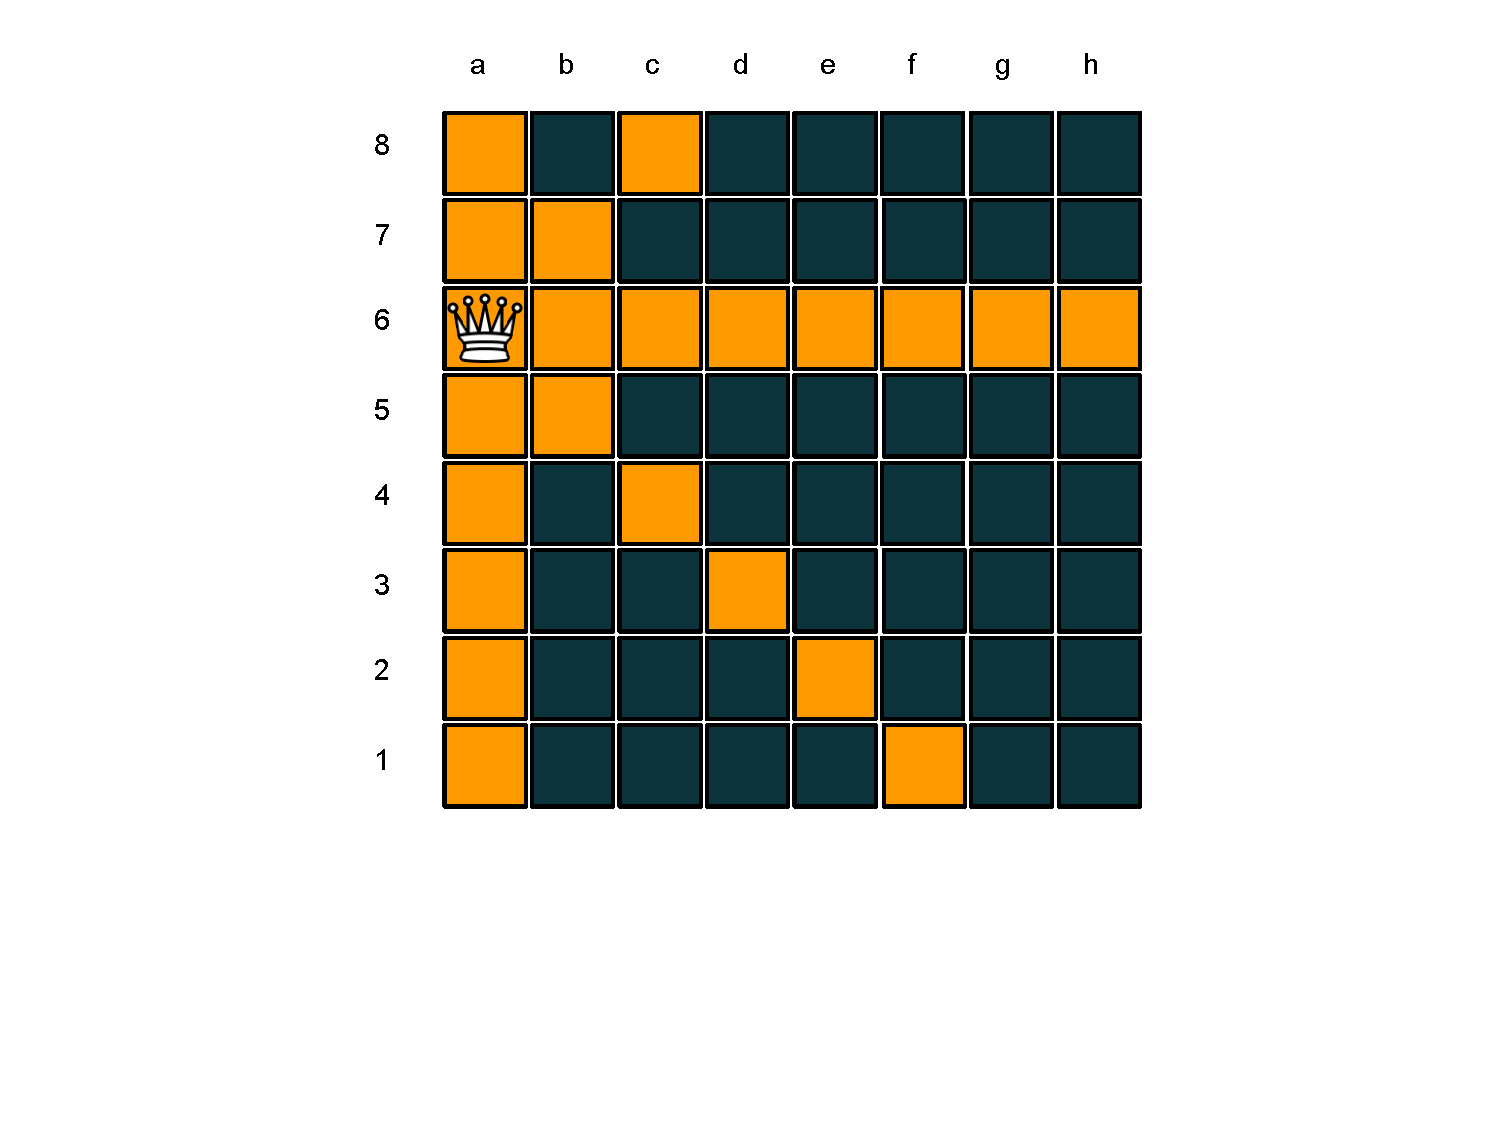
\includegraphics[width=12cm]{images/cb_0103}
\end{center}
\end{frame}


\begin{frame}[fragile]
\frametitle{Модел на играта}
\relscale{1}
\begin{lstlisting}
const int bs = 5;
bool board[bs][bs] = {false};
\end{lstlisting}
\end{frame}


\begin{frame}[fragile]
\frametitle{Модел на играта}
\relscale{0.8}
\begin{lstlisting}
void placeQueen (bool board[bs][bs], int row, int col)
{
  board[row][col] = true;
}
bool canPlaceQueen (bool board[bs][bs], int row, int col)
{
  for (int count = 0; count < bs; count++)
  {
    if (board[row][count] || board[count][col])
      return false;
  }
//....
\end{lstlisting}
\end{frame}



\begin{frame}[fragile]
\frametitle{(Обхождане на обратния диагонал)}
\begin{center}
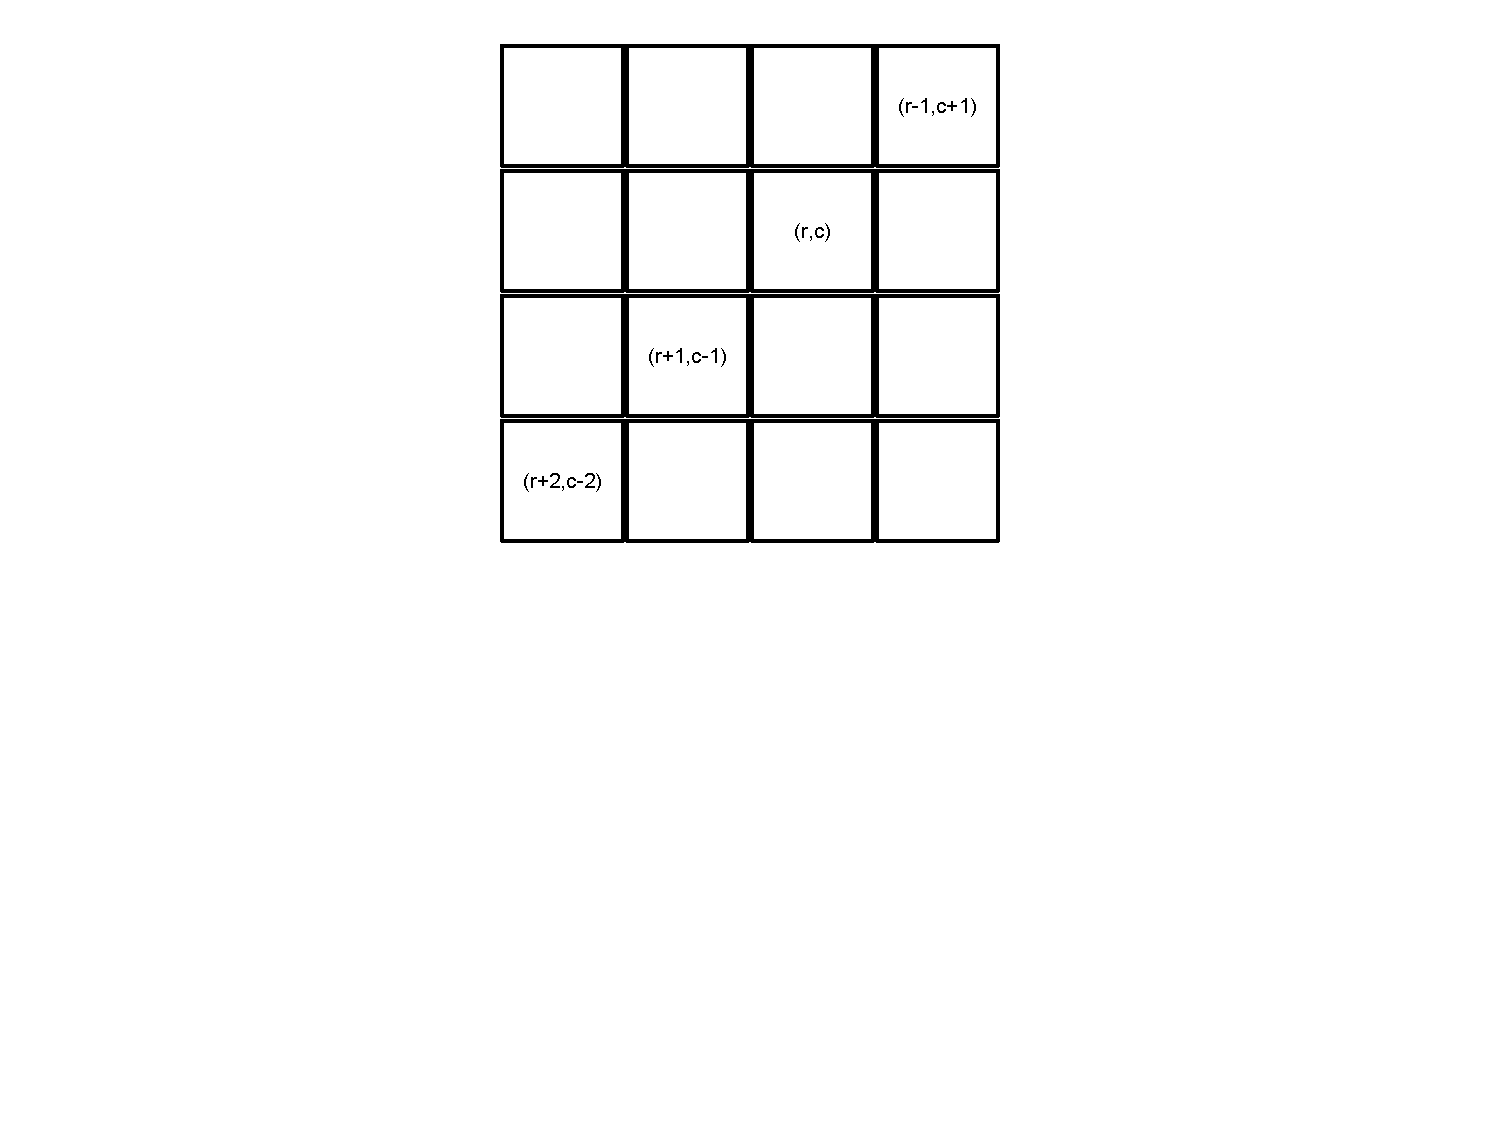
\includegraphics[width=12cm]{images/cb_count}
\end{center}
\vspace*{-125pt}
\begin{equation*}
(row+i,col-i), i = -1,..,2
\end{equation*}
\end{frame}


\begin{frame}[fragile]
\frametitle{(Обхождане на обратния диагонал)}
\begin{center}
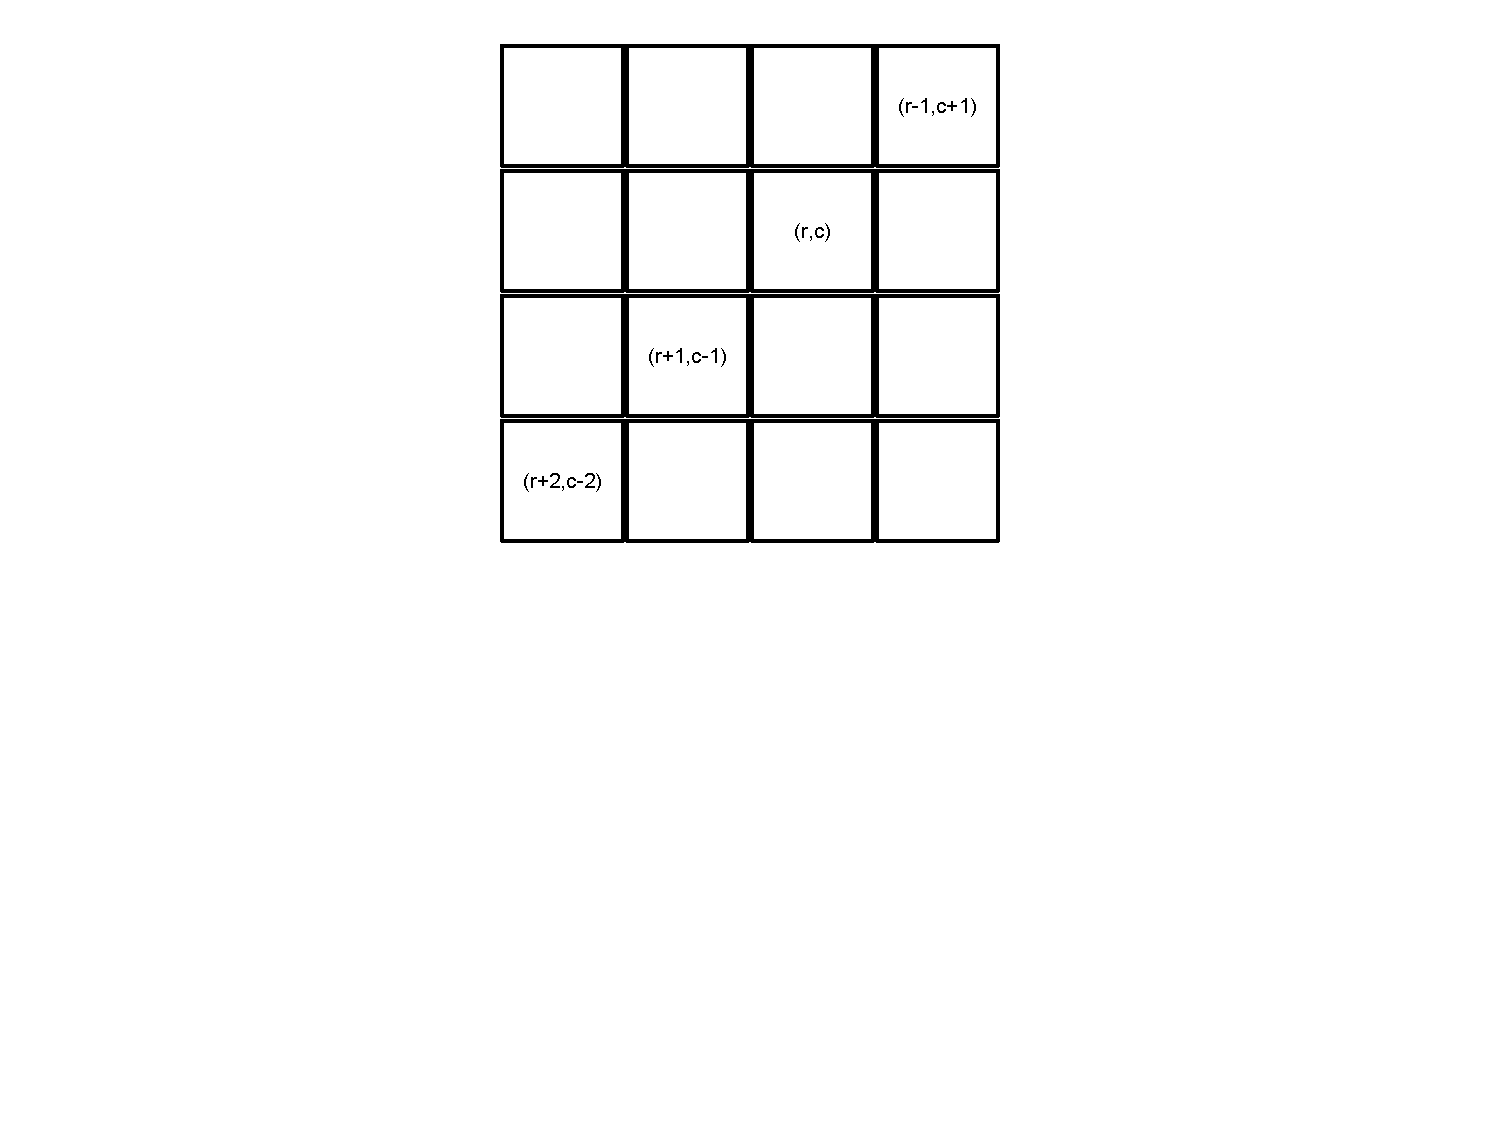
\includegraphics[width=12cm]{images/cb_count}
\end{center}
\vspace*{-150pt}

\begin{columns}[t]
  \begin{column}{0.3\textwidth}
$row+i > 0$

$row + i < 4$

$col-i > 0$

$col - i < 4$ 
  \end{column}
  \begin{column}{0.5\textwidth}
$i > -row$

$i < 4-row$

$i < col$

$i > col - 4$ 

  \end{column}

\end{columns}

\begin{center}
$i=max(-row,col-4),..,min (col,4-row)$
\end{center}

\end{frame}

\begin{frame}[fragile]
\frametitle{Модел на играта}

\begin{center}
$i=max(-row,col-bs),..,min (col,bs-row)$
\end{center}

\relscale{0.8}
\begin{lstlisting}
//....
  for (int count = -min(row,col); 
           count < min (bs-row,bs-col);
           count++)
  {
    if (board[row+count][col+count])
      return false;
  }
  for (int count = max(-row,col-bs); 
           count < min (col,bs-row);
           count++)
  {
    if (board[row+count][col-count])
      return false;
  }
  return true;
}
\end{lstlisting}


\end{frame}

\begin{frame}[fragile]
\frametitle{Връщане назад}
%\vspace*{-25pt}
\begin{center}
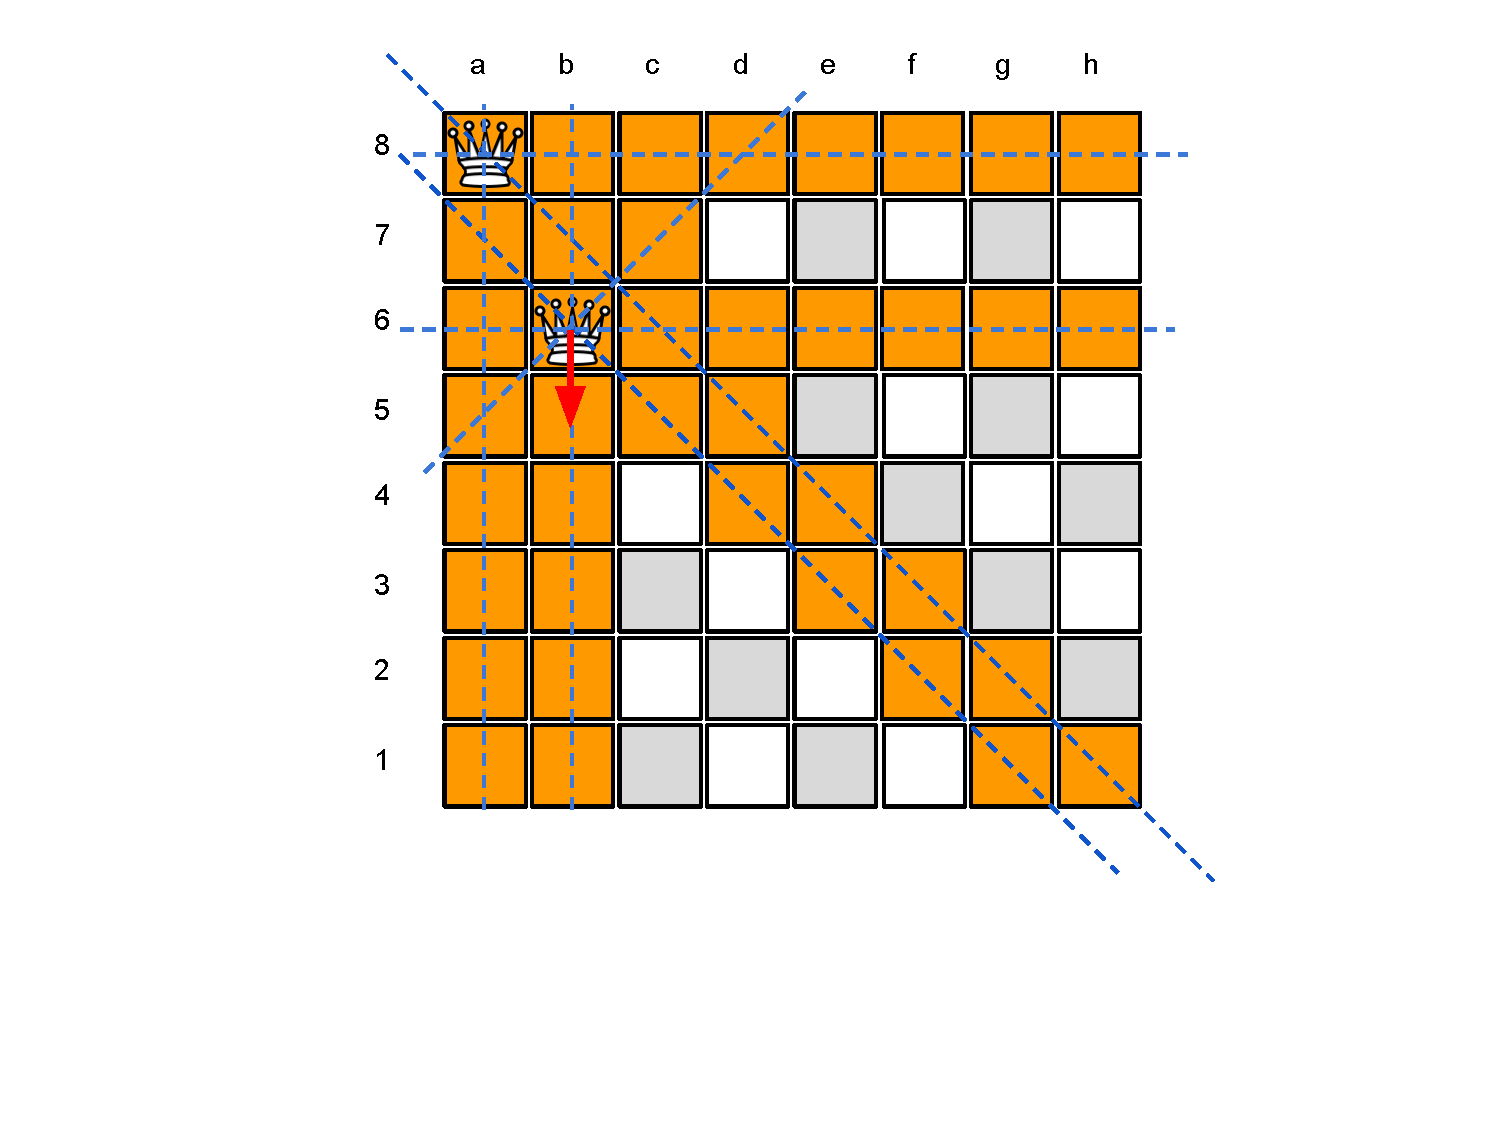
\includegraphics[width=12cm]{images/cb_choice_01}
\end{center}
\end{frame}


\begin{frame}[fragile]
\frametitle{Връщане назад}
%\vspace*{-25pt}
\begin{center}
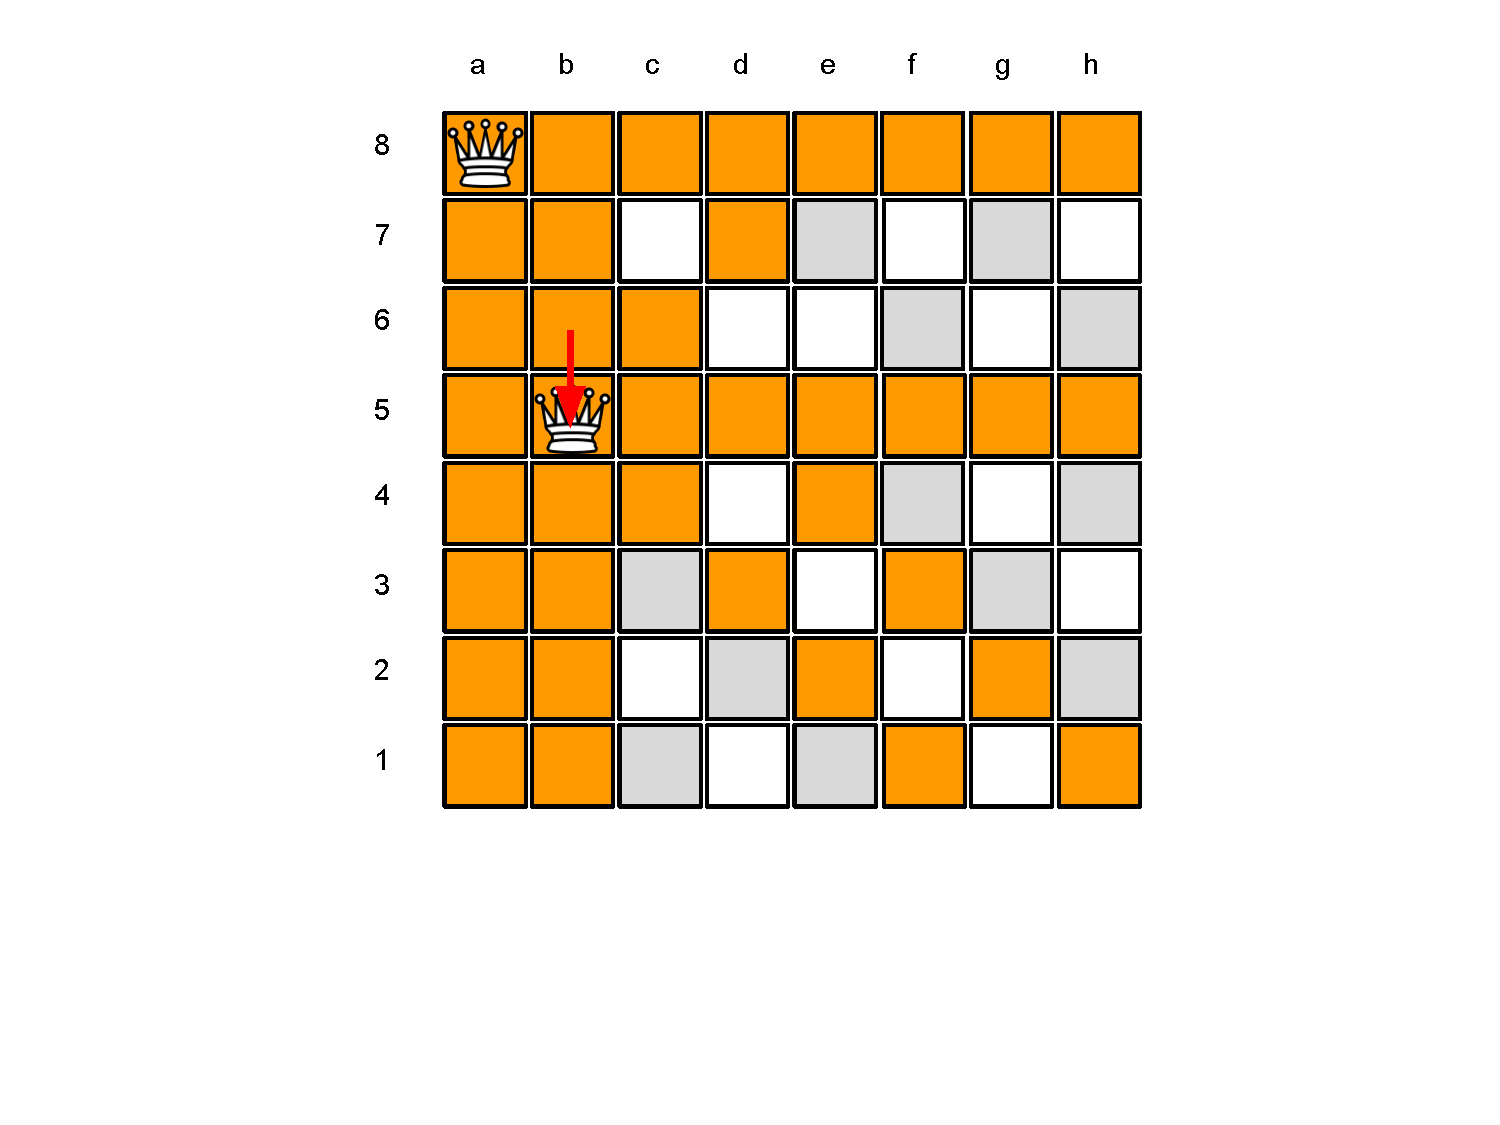
\includegraphics[width=12cm]{images/cb_choice_02}
\end{center}
\end{frame}


\begin{frame}[fragile]
\frametitle{Връщане назад}

\relscale{0.8}
\begin{lstlisting}
void replaceQueen (bool board[bs][bs], int row, int col)
{
  board[row][col] = false;
}
\end{lstlisting}
\end{frame}


\begin{frame}[fragile]
\frametitle{Проби и грешки}

\relscale{0.8}
\begin{lstlisting}
void placeQuuens (bool board[bs][bs], int number)
{
  if (number == 0)
  {
    printBoard(board);
    return;
  }
  for (int row = 0; row < bs; row++)
  {
    for (int col = 0; col < bs; col++)
    {
      if (canPlaceQueen (board,row,col))
      {
        placeQueen (board,row,col);
        placeQuuens (board,number-1);
        replaceQueen (board,row,col);
      }
    }
  }
}

\end{lstlisting}
\end{frame}

\begin{frame}
\centerline{Благодаря за вниманието!}
\end{frame}


\end{document}


\begin{columns}[t]
  \begin{column}{0.2\textwidth}

  \end{column}
  \begin{column}{0.8\textwidth}

  \end{column}
\end{columns}
